% ------------------------------------------------------------------
% The doubling theorem for bivariate bicycle codes — expository draft
% Audience: knows BB construction + group theory + basic ring theory;
% no analytic distance theory assumed.
% Build: pdflatex (twice for refs).
% ------------------------------------------------------------------
\documentclass[11pt]{article}

\usepackage[margin=1.05in]{geometry}
\usepackage{amsmath,amssymb,amsthm}
\usepackage{booktabs}
\usepackage{enumitem}
\usepackage{xcolor}
\usepackage{tikz}
\usetikzlibrary{arrows.meta,positioning,shapes.misc,patterns}
\usepackage[most]{tcolorbox}
\usepackage[colorlinks=true,linkcolor=blue!50!black,citecolor=blue!50!black,urlcolor=blue!50!black]{hyperref}

% ---------- theorem environments ----------
\theoremstyle{plain}
\newtheorem{theorem}{Theorem}[section]
\newtheorem{lemma}[theorem]{Lemma}
\newtheorem{proposition}[theorem]{Proposition}
\newtheorem{corollary}[theorem]{Corollary}
\theoremstyle{definition}
\newtheorem{definition}[theorem]{Definition}
\newtheorem{example}[theorem]{Example}
\theoremstyle{remark}
\newtheorem{remark}[theorem]{Remark}

% ---------- boxes ----------
\newtcolorbox{keyidea}[1][]{colback=blue!4!white,colframe=blue!45!black,
  fonttitle=\bfseries,title={#1},breakable,boxrule=0.6pt,left=6pt,right=6pt}
\newtcolorbox{inputbox}[1][]{colback=orange!6!white,colframe=orange!60!black,
  fonttitle=\bfseries,title={#1},breakable,boxrule=0.6pt,left=6pt,right=6pt}
\newtcolorbox{sloganbox}{colback=green!5!white,colframe=green!35!black,
  breakable,boxrule=0.6pt,left=6pt,right=6pt}

% ---------- macros ----------
\newcommand{\F}{\mathbb{F}}
\newcommand{\Z}{\mathbb{Z}}
\newcommand{\suppop}{\operatorname{supp}}
\newcommand{\Ann}{\operatorname{Ann}}
\newcommand{\imD}{\operatorname{im}\Delta}
\newcommand{\base}{\mathrm{base}}
\newcommand{\cov}{\mathrm{cover}}
\newcommand{\Rbase}{R}
\newcommand{\Rcov}{\widetilde{R}}
\newcommand{\wt}[1]{\lvert #1\rvert}

\title{\bfseries The doubling theorem for bivariate bicycle codes\\[4pt]
\large How the distance of a $2n$-qubit code reduces to finite checks on an
$n$-qubit code\\[6pt]
\normalsize\normalfont --- expository draft ---}
\author{}
\date{\today}

\begin{document}
\maketitle

\begin{abstract}
\noindent
The \emph{gross code} $[[144,12,12]]$ of Bravyi et al.\ is, in a precise sense,
two copies of a smaller bivariate bicycle (BB) code $[[72,12,6]]$ glued along a
cyclic direction of twice the length. The \emph{doubling theorem} says that this
gluing exactly doubles the distance: $d = 2\cdot 6 = 12$. More importantly, the
proof is a \emph{reduction}: instead of searching the 144-qubit code for
low-weight logical operators, one verifies a short list of concrete statements
about the 72-qubit code, plus a single one-line identity in a group algebra, and
the distance of the big code follows. This document develops the argument from
scratch for a reader who knows the BB construction, group theory, and basic ring
theory, but no ``distance technology.'' Everything except two clearly flagged
finite inputs is proved in full. We close with the general template, a gallery of
codes where doubling provably fails, and the list of verified instances,
including machine-checked (Lean) versions.
\end{abstract}

\tableofcontents

% ==================================================================
\section{Introduction}
% ==================================================================

For a stabilizer code, two of the three parameters $[[n,k,d]]$ are easy and one
is hard. The block length $n$ is read off the construction. The number of
logical qubits $k$ is linear algebra: a rank computation over $\F_2$. The
distance $d$ is different in kind. It is the minimum weight over all nontrivial
logical operators, and the set of logical operators is a union of exponentially
many cosets of the stabilizer group. There is no known way, in general, to
compute $d$ efficiently, and even for one fixed, moderately sized code, proving
a statement of the form ``\emph{no} logical operator has weight below $w$''
means excluding an astronomical number of candidates.

The bivariate bicycle (BB) codes of Bravyi, Cross, Gambetta, Maslov, Rall and
Yoder~\cite{bcgmry} made this concrete. Their headline code, the
\emph{gross code} $[[144,12,12]]$, had its distance determined by exhaustive
solver computation (mixed integer programming / SAT). At the time the research
program described here began, the best \emph{proof-style} lower bound applicable
to gross, due to Lin and Pryadko~\cite{linpryadko}, gave $d \geq 2$ --- a
factor of six below the truth.

This document is about a different route to $d(\mathrm{gross}) = 12$, found
and verified in the \texttt{qec-lab} and \texttt{QECLean} research program:
the \emph{doubling theorem}. The starting observation is structural. The gross code
is a BB code over the group $\Z_{12}\times\Z_6$, with polynomials
\[
A = x^3 + y + y^2, \qquad B = y^3 + x + x^2 .
\]
The \emph{same} polynomials also define a BB code over the smaller group
$\Z_6\times\Z_6$ --- a $[[72,12,6]]$ code we will call the \emph{base}. The
gross code is, in a sense made precise in Section~\ref{sec:cover}, a
\emph{double cover} of the base: two copies of the base's qubit grid, glued so
that the doubled direction wraps around twice. The doubling theorem says:

\begin{keyidea}[The doubling theorem, informally]
Under four checkable conditions on the base code and its polynomials, the
distance of the cover is exactly twice the distance of the base:
\[
d(\cov) \;=\; 2\, d(\base).
\]
For the gross code all four conditions hold, so $d(\mathrm{gross}) = 2\cdot 6 =
12$. The proof never searches the 144-qubit code: every condition is a finite,
concrete statement about the \emph{72-qubit} code, plus one polynomial identity.
\end{keyidea}

Why should you care, beyond the one value?

\begin{itemize}[leftmargin=2em]
\item \emph{It is a reduction, not a computation.} Distance proofs usually
  fight exponential search spaces. Here, the entire burden is shifted to the
  half-size code, where the remaining checks are small enough to survey --- and
  in the gross instance they were eventually carried out fully by hand and then
  machine-verified end to end in the Lean proof assistant.
\item \emph{The mechanism is portable.} The same template has produced verified
  instances over other groups, including a $[[300,8,16]]$ code whose distance
  theorem was obtained without any solver in the loop
  (Section~\ref{sec:instances}).
\item \emph{The failure modes are instructive.} Doubling is \emph{not}
  automatic --- the toric code is a counterexample, and the program found
  explicit BB codes where each condition individually fails
  (Section~\ref{sec:failures}). Understanding why the conditions are needed is
  understanding what makes gross special.
\end{itemize}

\paragraph{What we assume, and what we do not.}
We assume you know: the BB construction (group algebra $\F_2[G]$, two
polynomials, two blocks of qubits, the CSS check matrices); basic group theory
(quotients, cosets); and basic ring theory (ideals, quotient rings,
homomorphisms). We do \emph{not} assume familiarity with homology, covering
spaces, Fourier analysis on groups, or any prior distance-bounding technique.
Two hard finite facts about the base code are used as explicitly flagged black
boxes (they are theorems of the program, with precise statements and pointers);
everything else is proved in full, at a deliberate pace.

\paragraph{Reading map.}
Section~\ref{sec:setup} fixes notation and records the one duality lemma that
lets us work entirely with $Z$-type operators. Section~\ref{sec:cover}
constructs the cover and the two elementary maps --- \emph{fold} and
\emph{swap} --- that carry the whole argument. Section~\ref{sec:warmup} proves
a warm-up bound, $d(\mathrm{gross}) \geq 6$, and diagnoses exactly where it gets
stuck. Section~\ref{sec:liftfold} answers two innocent-looking questions
(``does a logical lift?'', ``does a logical fold?'') whose answers organize
everything that follows. Section~\ref{sec:architecture} lays out the proof
architecture. Sections~\ref{sec:dangerous} and~\ref{sec:safe} prove the two
halves of the lower bound, Section~\ref{sec:tightness} the matching upper
bound. Sections~\ref{sec:template}--\ref{sec:instances} give the general
template, the failure gallery, and the verified instances.

% ==================================================================
\section{Bivariate bicycle codes, on one side of the duality}
\label{sec:setup}
% ==================================================================

\subsection{Setup and notation}

Throughout, $G = \Z_\ell \times \Z_m$ is a finite abelian group, and
\[
\F_2[G] \;=\; \F_2[x,y]\,\big/\,(x^\ell = 1,\; y^m = 1)
\]
is its group algebra: polynomials in $x, y$ with coefficients $0$ or $1$,
multiplied with exponents reduced modulo $\ell$ and $m$. An element
$f \in \F_2[G]$ is the same data as a subset of $G$ (its \emph{support},
$\suppop f$); the \emph{weight} $\wt{f}$ is the number of monomials. We refer
to group elements/monomials as \emph{cells}, picturing $G$ as an
$\ell \times m$ grid that wraps around in both directions.

A BB code over $G$ with polynomials $A, B \in \F_2[G]$ has qubits
$L \sqcup R$, \emph{two} blocks each indexed by $G$, so $n = 2|G|$. A $Z$-type
Pauli operator is recorded as a pair
\[
v = (v_L, v_R), \qquad v_L, v_R \in \F_2[G],
\]
with $\wt{v} = \wt{v_L} + \wt{v_R}$, and similarly for $X$-type.

Elements of $\F_2[G]$ play two roles throughout, and it pays to keep them
straight. As a \emph{vector}, $f \in \F_2[G]$ is a formal sum of cells ---
its support --- and this is how we record Pauli patterns, one bit per qubit.
As a \emph{multiplier}, the same $f$ acts on vectors by ring multiplication,
$w \mapsto f\,w$, and this is how checks are built: $M_P$ denotes the matrix
of ``multiply by $P$,'' rows and columns indexed by cells. We write
$\delta_g$ for the monomial $x^a y^b$ attached to the cell $g = (a,b)$ ---
a ring element like any other, wearing both hats: as a vector it is the
basis vector supported on the single cell $g$; as a multiplier it
\emph{translates}, $\suppop(\delta_g\, w) = g + \suppop w$ (and $\delta_0 =
1$). Note $g$ itself is a group element, not a ring element; $\delta_g$ is
its avatar inside $\F_2[G]$. The check matrices are $H_X = (M_A \mid M_B)$
and $H_Z = (M_{B}^{\mathsf T} \mid M_{A}^{\mathsf T})$.

A word on the checks themselves, since everything below is phrased through
them. The \emph{checks} of a stabilizer code are its chosen stabilizer
generators --- the operators actually measured in each error-correction
round, as opposed to the full group they generate. For a CSS code each row
of $H_X$ is one $X$-check and each row of $H_Z$ is one $Z$-check. Both BB
check matrices have one row per element of $G$, so the checks --- like the
qubits --- are indexed by the cells of the grid: the \emph{$Z$-check at cell
$g$} means the row of $H_Z$ indexed by $g$, read as a $Z$-type Pauli
operator on the $2|G|$ qubits. (In the standard BB hardware layout, each
cell of the torus hosts four objects --- an $L$ data qubit, an $R$ data
qubit, an $X$ ancilla, and a $Z$ ancilla --- and the $Z$-check at $g$ is
what the $Z$ ancilla at cell $g$ measures.)

Only two derived maps matter in this document, and both are plain ring
multiplication. To see where they come from, unpack one row of $H_Z$. A row
of a transposed matrix is a column of the untransposed one, and the column
of a multiplication operator $M_P$ at position $g$ is the translate
$P\,\delta_g$. So, read as a $Z$-operator,
\[
\text{($Z$-check at cell $g$)} \;=\; \bigl(B\,\delta_g,\ A\,\delta_g\bigr)
\]
--- one fixed two-block pattern, ``$B$ on the $L$ block, $A$ on the $R$
block,'' stamped at position $g$. Concretely, with our polynomials: the check
at $g$ acts on the three $L$-qubits at $g + (0,3)$, $g + (1,0)$, $g + (2,0)$
(the support of $B$, translated by $g$) and the three $R$-qubits at
$g + (3,0)$, $g + (0,1)$, $g + (0,2)$ (the support of $A$, translated by
$g$) --- six qubits in all. A general element of the $Z$-stabilizer group is
a product of some \emph{set} of checks --- product in the \emph{Pauli
group}, not in the ring. Because $Z^2 = I$, multiplying $Z$-type Pauli
operators adds their exponent patterns mod 2 (the product acts by $Z$ on
exactly the qubits covered an odd number of times), so in the vector
encoding a Pauli product is an $\F_2$ \emph{sum}. Recording the set of
checks by its indicator $z \in \F_2[G]$ and summing the corresponding rows,
\[
\text{product of the checks in } z
\;=\; \sum_{g \,\in\, \suppop z} \bigl(B\,\delta_g,\ A\,\delta_g\bigr)
\;=\; \bigl(B\,z,\ A\,z\bigr),
\]
the last equality by distributivity. Note where ring multiplication enters:
between the fixed pattern and the indicator $z$ --- never between two
checks. That formula deserves a name, and the same bookkeeping on the $X$
side (pairing the rows of $H_X$ against a $Z$-operator) gives its companion:

\begin{definition}[syndrome and stabilizer maps]\label{def:CS}
The \emph{$X$-syndrome map} and the \emph{$Z$-stabilizer map} are
\[
C(v_L, v_R) := A\,v_L + B\,v_R \;\in\; \F_2[G],
\qquad
S(z) := (B\,z,\; A\,z) \;\in\; \F_2[G]^2 .
\]
\end{definition}

In words: $S(z)$ is \emph{the product of the $Z$-checks at the cells of $z$}
(Pauli product; $\F_2$ sum of rows). A single check is $S(\delta_g)$, and
the $Z$-stabilizer group is exactly $\operatorname{im} S$.

\begin{remark}[matrix dictionary]\label{rem:rowspace}
As length-$2|G|$ vectors, the $Z$-stabilizers form the \emph{row space} of
$H_Z$ --- in column conventions, $\operatorname{im} H_Z^{\mathsf T}$, and
\emph{not} $\operatorname{im} H_Z$, which is a space of syndromes living in
$\F_2^{|G|}$. Transposing the block matrix cancels the transposes inside it,
\[
H_Z^{\mathsf T} \;=\; \begin{pmatrix} M_B \\ M_A \end{pmatrix},
\qquad\text{so}\qquad
\operatorname{im} H_Z^{\mathsf T}
\;=\; \{\, (B\,z,\ A\,z) : z \in \F_2[G] \,\}
\;=\; \operatorname{im} S,
\]
with the polynomials appearing \emph{plain}, not inverted. (As an operator,
$M_B^{\mathsf T}$ is multiplication by the \emph{inverted} polynomial
$\iota(B)$, $g \mapsto -g$; if the stabilizers were $(\iota(B)z, \iota(A)z)$,
the commutation test would give $A\,\iota(B)z + B\,\iota(A)z \neq 0$ in
general, and CSS would fail. The transposes in $H_Z$'s definition are
pre-compensation: after the row-forming transpose undoes them, orthogonality
of $H_X$ and $H_Z$ becomes plain ring commutativity.)
\end{remark}

The companion map is read the other way around: $C(v)$ is the \emph{syndrome
polynomial} of the $Z$-operator $v$. Its coefficient at cell $g$ is the
commutation bit ($0$ = commute, $1$ = anticommute) of $v$ against the
$X$-check at $g$ --- a one-line check with the row description above --- so
$v$ commutes with every $X$-check if and only if $C(v) = 0$.

Notice that the two maps use the polynomials in \emph{opposite} blocks: $C$
pairs $(A, B)$ with $(L, R)$, while $S$ pairs $(B, A)$. The swap is not a
typo, and not a convention either --- it is exactly what makes stabilizers
invisible to the syndrome test, \emph{because $G$ is abelian}:
\[
C(S(z)) \;=\; A(Bz) + B(Az) \;=\; (AB + BA)\,z \;=\; 0 .
\]
Commutativity of the group is the CSS condition. Keep this computation in
mind; every ``chain map'' claim below is this computation in light disguise.

\subsection{Cycles, stabilizers, classes, distance}

\begin{definition}\label{def:cycles}
Fix a BB code as above. A \emph{cycle} is a $Z$-operator $v$ with $C(v) = 0$
(it commutes with all $X$-checks). A \emph{stabilizer} is an element of
$\operatorname{im} S$. Two cycles are \emph{equivalent} if they differ by a
stabilizer; an equivalence class is written $[v]$, and $[v] = 0$ means $v$ is
itself a stabilizer. A \emph{(nontrivial) logical} is a cycle with $[v] \neq
0$. The \emph{$Z$-distance} is
\[
d_Z \;=\; \min\{\, \wt{v} \;:\; v \text{ a cycle},\ [v] \neq 0 \,\}.
\]
\end{definition}

Because everything in sight is $\F_2$-linear, the classes themselves form a
vector space --- the quotient of the cycles by the stabilizers --- which we
call the \emph{class space}. A standard rank count identifies its dimension
with $k$, the number of logical qubits: $12$ for both of our codes, so each
has $2^{12}$ classes, $2^{12} - 1$ of them nonzero. How classes move between
the two codes will become the organizing question of the proof
(Section~\ref{sec:liftfold}).

The distance is a minimum over equivalence classes: to bound it from below you
must argue about \emph{every} representative of \emph{every} nonzero class,
which is what makes such proofs hard; to bound it from above you exhibit one
cycle and certify that its class is nonzero, which is subtler than it looks
(certifying \emph{non}-membership in a $2^{|G|}$-element subspace).

One notational convention, used heavily from Section~\ref{sec:dangerous}
on. The \emph{support} of a $Z$-operator $v = (v_L, v_R)$ is
$\suppop v := \suppop v_L \sqcup \suppop v_R$, a set of \emph{qubit}
positions in $L \sqcup R$ (an $L$-position and an $R$-position with the
same grid coordinates are different qubits). For a set $T$ of positions,
``$f$ off $T$'' means the restriction of $f$ to positions outside $T$
(zero out $T$, keep the rest), so that
\[
\wt{f \text{ off } T} \;=\; \lvert \suppop f \setminus T \rvert ,
\]
the comparison running blockwise --- $L$ against $L$, $R$ against $R$.

\subsection{The \texorpdfstring{$X$--$Z$}{X-Z} duality: one side suffices}

BB codes have an exact symmetry exchanging the two Pauli types.

\begin{lemma}[inversion duality]\label{lem:duality}
Let $\iota : \F_2[G] \to \F_2[G]$ be the linear extension of inversion,
$\iota(x^ay^b) = x^{-a}y^{-b}$. Then
\[
\Phi(w_L, w_R) := (\iota(w_R),\, \iota(w_L))
\]
is a weight-preserving linear bijection that maps $X$-cycles to $Z$-cycles and
$X$-stabilizers to $Z$-stabilizers. Consequently $d_X = d_Z$.
\end{lemma}

\begin{proof}
Since $G$ is abelian, $\iota$ is a ring automorphism of $\F_2[G]$. The
$X$-side objects are the mirror images of Definition~\ref{def:CS} with the
roles of $A, B$ transposed through $\iota$: an $X$-operator $w$ commutes with
all $Z$-checks iff $\iota(B) w_L + \iota(A) w_R = 0$, and the $X$-stabilizers
are generated by $(\iota(A) z, \iota(B) z)$. Apply $\iota$ to these equations
and swap the two blocks; they become exactly $C(\Phi(w)) = 0$ and
$\Phi(\text{$X$-stab}) = S(\iota(z))$. $\Phi$ clearly preserves weight, and
$\Phi^2 = \mathrm{id}$.
\end{proof}

From now on \emph{every} operator in this document is $Z$-type, and ``the
distance'' means $d_Z$; Lemma~\ref{lem:duality} silently gives the $X$-side
statements for free.

\subsection{The running example}

Our running pair, with $A = x^3 + y + y^2$ and $B = y^3 + x + x^2$ throughout:

\begin{center}
\begin{tabular}{lllll}
\toprule
 & group & ring & parameters & role\\
\midrule
base & $\Z_6 \times \Z_6$ & $\Rbase = \F_2[x,y]/(x^{6}{=}1,\,y^{6}{=}1)$ &
$[[72,12,6]]$ & the small code\\
cover & $\Z_{12} \times \Z_6$ & $\Rcov = \F_2[x,y]/(x^{12}{=}1,\,y^{6}{=}1)$ &
$[[144,12,12]]$ & the gross code\\
\bottomrule
\end{tabular}
\end{center}

Note what is \emph{not} changing: the polynomials, the $y$-direction, the
number of logical qubits. Only the $x$-direction doubles. That $k$ stays at
$12$ looks like a curiosity now; by Section~\ref{sec:template} it will turn out
to be \emph{equivalent} to the linchpin condition of the whole proof.

% ==================================================================
\section{The double cover: fold and swap}
\label{sec:cover}
% ==================================================================

\subsection{Reduce mod 6}

Everything in this section is elementary group theory applied to one map.
There is a surjective homomorphism
\[
\pi : \Z_{12} \to \Z_6, \qquad a \mapsto a \bmod 6,
\]
with kernel $\{0, 6\}$. Applying it to the first coordinate gives
\[
\pi : \Z_{12}\times\Z_6 \;\to\; \Z_6\times\Z_6, \qquad
(a, b) \mapsto (a \bmod 6,\; b).
\]
Because the kernel has size two, \textbf{every base cell has exactly two
preimages}: the preimages of $(a,b)$ are $(a,b)$ and $(a{+}6,\,b)$. That is the
entire content of the phrase ``double cover.'' (Analogy: read a 12-hour clock
hand on a 6-hour dial. Positions $3$ and $9$ both display as ``3''; one trip
around the 12-dial passes over the 6-dial twice.)

Write each $a \in \Z_{12}$ uniquely as $a = r + 6s$ with $r \in \{0,\dots,5\}$
and $s \in \{0,1\}$: then $r$ says \emph{where you land} downstairs and $s$
says \emph{which copy} you are in. We call the two copies \emph{sheets}.
Figure~\ref{fig:sheets} shows the picture: the cover's $12\times 6$ grid is
two aligned $6\times 6$ copies of the base grid, and a vector over the cover
is the same data as a \emph{pair} of base vectors,
\[
v \;\longleftrightarrow\; (v_0,\, v_1)
\qquad\text{(restriction to sheet 0 and sheet 1).}
\]
From here on we freely say \emph{upstairs} for the cover and
\emph{downstairs} for the base.

\begin{figure}[ht]
\centering
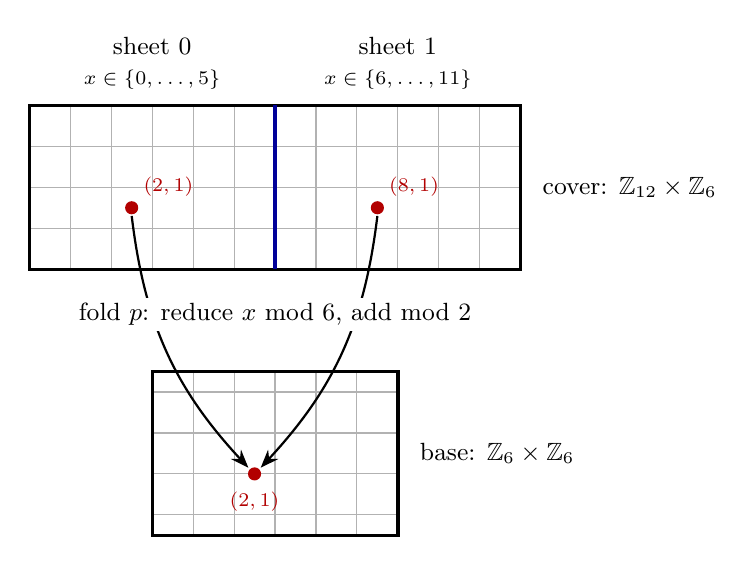
\begin{tikzpicture}[scale=0.52]
% cover grid
\draw[step=1,gray!60,thin] (0,0) grid (12,4);
\draw[very thick] (0,0) rectangle (12,4);
\draw[very thick,blue!60!black] (6,0) -- (6,4);
\node[anchor=south, align=center] at (3,4.15)
  {\small sheet $0$\\[-1pt] \scriptsize $x\in\{0,\dots,5\}$};
\node[anchor=south, align=center] at (9,4.15)
  {\small sheet $1$\\[-1pt] \scriptsize $x\in\{6,\dots,11\}$};
\node[anchor=west] at (12.3,2) {\small cover: $\Z_{12}\times\Z_6$};
% highlighted pair of cells
\fill[red!70!black] (2.5,1.5) circle (0.16);
\fill[red!70!black] (8.5,1.5) circle (0.16);
\node[red!70!black,anchor=south west] at (2.55,1.55) {\scriptsize $(2,1)$};
\node[red!70!black,anchor=south west] at (8.55,1.55) {\scriptsize $(8,1)$};
% base grid
\draw[step=1,gray!60,thin] (3,-6.5) grid (9,-2.5);
\draw[very thick] (3,-6.5) rectangle (9,-2.5);
\node[anchor=west] at (9.3,-4.5) {\small base: $\Z_{6}\times\Z_6$};
\fill[red!70!black] (5.5,-5) circle (0.16);
\node[red!70!black,anchor=north] at (5.5,-5.2) {\scriptsize $(2,1)$};
% fold arrows
\draw[-{Stealth},thick] (2.5,1.3) to[bend right=18] (5.35,-4.85);
\draw[-{Stealth},thick] (8.5,1.3) to[bend left=18] (5.65,-4.85);
\node[fill=white, inner sep=2pt] at (6,-1.1)
  {\small fold $p$: reduce $x$ mod $6$, add mod $2$};
\end{tikzpicture}
\caption{The cover as two sheets over the base. Both marked cover cells sit
over the same base cell; if a vector contains both, they cancel when folded.}
\label{fig:sheets}
\end{figure}

\subsection{The two maps, in ring language}

Two maps organize the whole story, and both have one-line descriptions in
$\Rcov$:

\begin{definition}[fold and swap]\label{def:foldswap}
\leavevmode
\begin{itemize}[leftmargin=2em]
\item The \emph{fold} $p : \Rcov \to \Rbase$ is the ring homomorphism that
  imposes $x^6 = 1$: each monomial $x^a y^b \mapsto x^{a \bmod 6} y^b$, with
  coefficients added mod 2. In sheet coordinates, $p(v) = v_0 + v_1$. We call
  $p(v)$ the \emph{shadow} of $v$.
\item The \emph{swap} $\sigma : \Rcov \to \Rcov$ is multiplication by the
  monomial $x^6$: it adds $6$ to every $x$-exponent. In sheet coordinates,
  $\sigma(v_0, v_1) = (v_1, v_0)$.
\end{itemize}
Both maps act on $Z$-operators blockwise: $p(v_L, v_R) = (p\,v_L,\, p\,v_R)$,
and likewise $\sigma$.
\end{definition}

\begin{remark}[two pairings, kept apart]\label{rem:twopairs}
A cover $Z$-operator carries \emph{two} independent two-fold structures,
both written as ordered pairs, and they must not be conflated. The
\emph{block} pair $v = (v_L, v_R)$ sorts qubits into the blocks $L$ and $R$;
both codes have it, and no map in this document ever adds one block to the
other. The \emph{sheet} pair $f \leftrightarrow (f_0, f_1)$ decomposes a
single ring element of the cover by its $x$-exponent range; only the cover
has it, and \emph{this} is the pair the fold sums. In full coordinates a
cover operator is a $2 \times 2$ array, and the fold sums along the sheet
axis only:
\[
v = \bigl( (v_L)_0, (v_L)_1 \,;\; (v_R)_0, (v_R)_1 \bigr),
\qquad
p(v) = \bigl( (v_L)_0 + (v_L)_1,\;\; (v_R)_0 + (v_R)_1 \bigr).
\]
So, for instance, $p(B\,\widetilde z,\ A\,\widetilde z) =
\bigl(p(B\widetilde z),\, p(A\widetilde z)\bigr)$ --- it is \emph{not}
$B\widetilde z + A\widetilde z$; adding the $L$ block to the $R$ block is no
operation of ours. (When a cover operator is written $(v_0, v_1)$ below,
each entry is a full block pair, $v_i = ((v_L)_i, (v_R)_i)$.)
\end{remark}

The swap deserves three one-line observations. It has order two ($x^6 \cdot
x^6 = x^{12} = 1$). It moves \emph{every} cell ($a + 6 \not\equiv a \bmod
12$) --- one says the action is \emph{free}; contrast negation $a \mapsto -a$,
also of order two, which fixes $0$ and $6$ and therefore does \emph{not} split
$\Z_{12}$ into two interchangeable copies. And it commutes with everything in
sight, being multiplication by a ring element. In covering-space language
$\sigma$ is called the \emph{deck transformation}; we will mostly say
``swap.''

Because $A$ and $B$ only use $x$-exponents below 6, \textbf{the identical
polynomial expressions define both codes}, and
\[
p(A) = A, \qquad p(B) = B.
\]
Since $p$ is a ring homomorphism, it follows at once that
\begin{equation}\label{eq:chainmap}
p(A f) = A\, p(f), \qquad p(B f) = B\, p(f) \qquad (f \in \Rcov),
\end{equation}
that is, \emph{folding commutes with all check operations}. This innocuous
line is doing real work: it is the entire ``compatibility of the two codes.''

\subsection{The diagonal lemma}

Vectors that look the same on both sheets play a starring role.

\begin{definition}
A cover vector $v$ is \emph{diagonal} if $v_0 = v_1$. For a base vector $u$,
the \emph{diagonal lift} is
\[
\tau(u) := (u, u) \;=\; (1 + x^6)\cdot \widetilde u,
\]
where $\widetilde u$ is the copy of $u$ drawn on sheet 0, i.e.\ written with
$x$-exponents in $\{0,\dots,5\}$ only. We call $\widetilde u$ the
\emph{exponent-restricted lift} of $u$; note $p(\widetilde u) = u$. (Both
descriptions define the same vector $\tau(u)$; the second shows $\tau$ is
built from ring operations.) Note $\wt{\tau(u)} = 2\wt{u}$.
\end{definition}

\begin{remark}[tilde conventions]\label{rem:tilde}
Tildes always mean \emph{upstairs}. On the ring and the maps ($\Rcov$,
$\widetilde C$, $\widetilde S$) a tilde marks the cover version. On an
element it marks residence in the cover ring; when the untilded symbol names
a base element, as in $\widetilde u$ or $\widetilde\zeta$, it means
specifically the exponent-restricted lift --- \emph{the same formal
expression, re-read in the bigger ring}. (Occasionally a tilde decorates a
fresh variable, as in ``for some $\widetilde z \in \Rcov$''; there it only
signals where the variable lives.) Beware what the lift is \emph{not}: it is
$\F_2$-linear with $p(\widetilde u) = u$, but it is not a ring homomorphism,
and no linear section of $p$ can be one. Downstairs $x^5 \cdot x = x^6 = 1$;
lift each factor and multiply upstairs and you get $x^6 \neq 1$.
Multiplication that wraps around downstairs fails to wrap upstairs, and the
discrepancy is always a multiple of $1 + x^6$ (the two products share a
shadow, so they differ by an element of $\ker p$). Much of
Section~\ref{sec:liftfold} consists of harvesting this failure.
\end{remark}

\begin{lemma}[diagonal lemma]\label{lem:diagonal}
For $f \in \Rcov$ (or blockwise for $Z$-operators), the following are
equivalent:
\emph{(i)} $f$ is diagonal;\quad
\emph{(ii)} $f$ is a multiple of $1 + x^6$;\quad
\emph{(iii)} $(1+x^6)\,f = 0$;\quad
\emph{(iv)} $p(f) = 0$.
Moreover, for every $f \in \Rcov$,
\begin{equation}\label{eq:master}
(1 + x^6)\, f \;=\; f + \sigma f \;=\; \tau\bigl(p(f)\bigr)
\qquad \text{(\emph{the master identity}).}
\end{equation}
\end{lemma}

\begin{proof}
First the master identity, which is pure sheet bookkeeping: with $f = (f_0,
f_1)$,
\[
f + \sigma f = (f_0, f_1) + (f_1, f_0) = (f_0 + f_1,\; f_0 + f_1)
= \tau(f_0 + f_1) = \tau(p(f)),
\]
and $f + \sigma f = (1 + x^6) f$ because $\sigma$ is multiplication by $x^6$.

Now the equivalences. (i)$\Leftrightarrow$(iv): $p(f) = f_0 + f_1 = 0$ iff
$f_0 = f_1$. (i)$\Leftrightarrow$(iii): by the master identity, $(1+x^6)f =
\tau(p(f))$, which vanishes iff $p(f) = 0$. (i)$\Rightarrow$(ii): if $f =
(f_0, f_0)$ then $f = (1+x^6)\widetilde{f_0}$. (ii)$\Rightarrow$(iv): $p(1 +
x^6) = 1 + 1 = 0$ and $p$ is a ring map.
\end{proof}

\begin{remark}
Item (ii)$\Leftrightarrow$(iii) says: in $\Rcov$, the kernel of multiplication
by $(1+x^6)$ \emph{equals} its image. You may enjoy checking this is the
statement that $(1+x^6)^2 = 1 + x^{12} = 0$ --- the characteristic-2 Frobenius
--- together with a dimension count; we only ever use the four equivalences
above.
\end{remark}

\subsection{Worked examples of folding}

Suppress $y$ for a moment (it comes along for the ride) and fold three small
vectors:

\begin{center}
\begin{tabular}{llll}
\toprule
cover vector $v$ & sheets $(v_0, v_1)$ & shadow $p(v)$ & weight\\
\midrule
$x^2 + x^7$ & $(x^2,\ x)$ & $x^2 + x$ & $2 \to 2$ \ preserved\\
$x^2 + x^8$ & $(x^2,\ x^2)$ & $0$ & $2 \to 0$ \ collapses\\
$x^2 + x^3 + x^8$ & $(x^2{+}x^3,\ x^2)$ & $x^3$ & $3 \to 1$ \ partial\\
\bottomrule
\end{tabular}
\end{center}

The middle row is the one to remember: $x^2$ and $x^8$ are the two preimages
of the same base cell, so they cancel mod 2. Notice $x^2 + x^8 =
(1+x^6)\,x^2 = \tau(x^2)$: a diagonal vector, invisible to the fold, of weight
exactly twice that of its base half --- Lemma~\ref{lem:diagonal} in its
smallest instance.

\subsection{Folding respects the code structure}

We can now record, with complete proofs, the elementary facts that power the
whole argument. To distinguish the two levels we write $\widetilde C,
\widetilde S$ for the cover's syndrome/stabilizer maps and $C, S$ for the
base's (same formulas, different rings).

\begin{lemma}[transport facts]\label{lem:transport}
\leavevmode
\begin{enumerate}[label=\emph{(\arabic*)},leftmargin=2.4em]
\item \emph{Fold.} $p$ maps cover cycles to base cycles and cover stabilizers
  to base stabilizers. Hence $p$ descends to classes: $[v] \mapsto [p(v)]$ is
  well defined.
\item \emph{Weight.} $\wt{v} \geq \wt{p(v)}$ for every cover operator $v$.
\item \emph{Diagonal.} $p(v) = 0$ iff $v = \tau(u)$ for some base operator
  $u$; and $\tau(u)$ is a cover cycle iff $u$ is a base cycle; in that case
  $\wt{\tau(u)} = 2\wt{u}$.
\item \emph{Lift of stabilizers.} $\tau$ maps base stabilizers to cover
  stabilizers.
\end{enumerate}
\end{lemma}

\begin{proof}
(1) If $\widetilde C(v) = A v_L + B v_R = 0$, apply the ring homomorphism $p$
and use~\eqref{eq:chainmap}: $C(p(v)) = A\,p(v_L) + B\,p(v_R) = p(\widetilde
C(v)) = 0$. Similarly, blockwise (Remark~\ref{rem:twopairs}),
$p(\widetilde S(z)) = p(Bz, Az) = \bigl(p(Bz),\, p(Az)\bigr) =
(B\,p(z),\, A\,p(z)) = S(p(z))$.

(2) Each base cell receives the mod-2 sum of the values on its two preimages;
a sum of two bits has weight at most the number of ones among them.

(3) The first claim is Lemma~\ref{lem:diagonal}(i)$\Leftrightarrow$(iv),
blockwise. For the second: $\widetilde C(\tau(u)) = \widetilde
C((1+x^6)\widetilde u) = (1+x^6)\,\widetilde C(\widetilde u)$, and by
Lemma~\ref{lem:diagonal} this vanishes iff $p(\widetilde C(\widetilde u)) =
0$; but $p(\widetilde C(\widetilde u)) = C(p(\widetilde u)) = C(u)$ by
\eqref{eq:chainmap}.

(4) $\tau(S(z)) = (1+x^6)\cdot\widetilde{S(z)}$. Now $\widetilde S(\widetilde
z)$ is a cover vector folding to $S(z)$, so $\widetilde{S(z)}$ and $\widetilde
S(\widetilde z)$ differ by an element of $\ker p = \operatorname{im}(1+x^6)$
(Lemma~\ref{lem:diagonal}); multiplying by $(1+x^6)$ kills that difference
(as $(1+x^6)^2 = 0$), so
$\tau(S(z)) = (1+x^6)\,\widetilde S(\widetilde z) = \widetilde
S\bigl((1+x^6)\widetilde z\bigr) \in \operatorname{im}\widetilde S$.
\end{proof}

Pause on what these four facts \emph{feel} like. The fold sees the code
structure perfectly (1), can only lose weight (2), and is blind to exactly the
diagonal vectors, which cost double (3). Everything so far is formal --- true
for \emph{any} BB code and \emph{any} doubled direction, with no hypotheses.
The theorem-quality content starts when we ask how much weight the fold can
lose, and for that we need to know something real about the base code.

% ==================================================================
\section{A warm-up bound, and the wall at \texorpdfstring{$d$}{d}}
\label{sec:warmup}
% ==================================================================

\subsection{Input 1: the base code has no small cycles}

Here is the first of the two black-box inputs. Note carefully that it speaks
about \emph{cycles}, not just logicals: stabilizers are included.

\begin{inputbox}[Input (T-A): no small cycles in the base]
\textbf{Theorem A} (proved in the program's write-up, fully by hand). The base
code $[[72,12,6]]$ has no nonzero cycle of weight $\leq 5$: every nonzero
$v = (v_L, v_R)$ with $A v_L + B v_R = 0$ has $\wt{v} \geq 6$. In particular
$d(\base) \geq 6$, and every nonzero stabilizer has weight $\geq 6$.
\end{inputbox}

Two remarks so this box does not feel like magic. First, a taste of the proof,
which is a finite case analysis over the possible weight splits
$(\wt{v_L}, \wt{v_R})$. Its basic tool recurs throughout the document (the
D-pairs of Section~\ref{sec:dangerous} are built from it), so we give it a
numbered home:

\begin{definition}[difference sets]\label{def:diffsets}
The \emph{difference sets} of the polynomials are
\[
dA := \{\,g - h \;:\; g \neq h \in \suppop A\,\}, \qquad
dB := \{\,g - h \;:\; g \neq h \in \suppop B\,\}.
\]
For our $A, B$ one computes
$dA = \{(0,{\pm}1), (3,{\pm}1), (3,{\pm}2)\}$ and
$dB = \{({\pm}1,0), ({\pm}1,3), ({\pm}2,3)\}$, and two properties are read
off the computation. The two sets are \emph{disjoint}. And each has six
elements arising from the six ordered pairs, so every difference arises
from \emph{exactly one} pair --- one says the difference sets are
\emph{multiplicity-free}; consequently two translates $B\delta_g$ and
$B\delta_h$ ($g \neq h$) overlap in at most one cell (an overlap cell
corresponds to a pair of $\suppop B$ with difference $g - h$), and in
exactly one cell iff $g - h \in dB$ (mirror statement for $A$).
\end{definition}

Now suppose a cycle had weight split $(1,1)$: $A\, x^{g} = B\, x^{h}$ (single cells on both
sides). Two translates of $\suppop A$ and $\suppop B$ would then be
\emph{equal} as 3-element sets, forcing their difference sets to coincide:
$dA = dB$. But they are disjoint and nonempty --- contradiction. The other
splits die by similar, longer elimination games with these difference sets
(the largest case table in the full proof has nine entries). Second, the
statement is exactly sharp: the explicit weight-6 element
\begin{equation}\label{eq:ustar}
u^* \;=\; \bigl(z^*,\, 0\bigr), \qquad
z^* = 1 + y + y^2 + y^5 + x^3 + x^3y^4
\end{equation}
satisfies $A z^* = 0$ (check it: six cancellations) and is a nontrivial
logical, so $d(\base) = 6$.

\subsection{The projection bound}

\begin{theorem}[warm-up]\label{thm:warmup}
Every nonzero cycle of the cover has weight $\geq 6$. In particular
$d(\mathrm{gross}) \geq 6$.
\end{theorem}

\begin{proof}
Let $v \neq 0$ be a cover cycle and consider its shadow.

\emph{Case 1: $p(v) \neq 0$.} By Lemma~\ref{lem:transport}(1), $p(v)$ is a
nonzero base cycle, so $\wt{v} \geq \wt{p(v)} \geq 6$ by
Lemma~\ref{lem:transport}(2) and Input (T-A).

\emph{Case 2: $p(v) = 0$.} By Lemma~\ref{lem:transport}(3), $v = \tau(v_0)$
with $v_0$ a nonzero base cycle, so $\wt{v} = 2\wt{v_0} \geq 12$.
\end{proof}

Modest as it looks, this already \emph{tripled} the best previously published
proof-style bound for gross ($d \geq 2$). But it stalls at $6 = d(\base)$, and
the post-mortem tells us exactly why. Case 2 is great: diagonal candidates pay
double. Case 1 is the bottleneck: a shadow can be nonzero yet cost only
$d(\base)$. If we want $2d$, we must extract more from Case 1 --- and the only
information we are using about the shadow is that it is a nonzero
\emph{vector}. The move that unlocks everything is to ask about the shadow's
\emph{class}.

\begin{keyidea}[The refinement]
Sort a candidate logical $v$ not by whether $p(v) = 0$ as a vector, but by
whether $[p(v)] = 0$ as a class --- i.e.\ whether the shadow is a stabilizer
(possibly zero) or a genuine base logical. Each alternative will get its own
mechanism forcing weight $\geq 2d$.
\end{keyidea}

Before building those mechanisms, we need to understand how logicals interact
with lifting and folding \emph{at the level of classes}. That is the next
section, and it is the conceptual heart of the paper.

% ==================================================================
\section{Lifting and folding: two questions}
\label{sec:liftfold}
% ==================================================================

The refinement at the end of Section~\ref{sec:warmup} wants candidate
logicals sorted by the \emph{class} of their shadow. Before that plan can
bear weight, we need to understand how logical classes move between the two
codes at all --- and the traffic runs in both directions: base classes can
be lifted diagonally ($\tau$), cover classes can be folded down ($p$). This
section asks the two natural questions about that traffic, and both get the
same answer: \emph{not always --- and the exceptions are structured}. The
two exceptional sets uncovered here are the central objects of the entire
proof: a subspace $\imD$ of base classes, which will confine the safe
sector (Section~\ref{sec:safe}) and certify the tightness witness
(Section~\ref{sec:tightness}); and a family of cover classes which
\emph{is} the dangerous sector (Section~\ref{sec:dangerous}).

\subsection{Does a base logical lift?}
\label{sec:lift}

Let $u$ be a nontrivial base logical of weight $w$. Its diagonal lift
$\tau(u)$ is a cover cycle of weight $2w$ (Lemma~\ref{lem:transport}(3)),
and one would love it to be a nontrivial cover \emph{logical}: applied to a
minimum-weight base logical ($w = d(\base)$), that would exhibit a cover
logical of weight $2\,d(\base)$ and hand us the upper-bound half of the
theorem, $d(\cov) \leq 2\,d(\base)$. So: is the diagonal lift of a logical
always a logical?

\textbf{Not necessarily} --- and rather than pull the obstruction out of a
hat, we can let the question point to it. Asking whether $\tau(u)$ is a
cover stabilizer means asking whether the equation
\[
\tau(u) \;=\; \widetilde S(\widetilde w)
\]
has a solution $\widetilde w \in \Rcov$. Apply the fold to both sides. The
left side folds to zero --- diagonal vectors have zero shadow
(Lemma~\ref{lem:diagonal}) --- while the right side folds to
$S(p(\widetilde w))$ (Lemma~\ref{lem:transport}(1)). So any $\widetilde w$
that manufactures a diagonal stabilizer is constrained: its own shadow must
be annihilated by the base stabilizer map,
\[
p(\widetilde w) \;\in\; \ker S
\;=\; \{\, \zeta \in \Rbase \;:\; B\zeta = A\zeta = 0 \,\}
\;=\; \Ann(A) \cap \Ann(B) \;=:\; K,
\]
where $\Ann(f) := \{\, g : f g = 0 \,\}$ is the annihilator ideal of $f$.
The subspace $K$ --- the base elements killed by \emph{both} polynomials ---
is forced on us by the question, not chosen. And it helps to hear what
membership in $K$ says: $S(\zeta) = 0$ means the product of the $Z$-checks
over the cells of $\zeta$ is the \emph{identity} --- $\zeta$ encodes a
\emph{relation} (a redundancy) among the base checks. (The single-shot
error-correction literature calls such relations \emph{metachecks}.) For
gross's base the relation space is genuinely inhabited: $\dim_{\F_2} K = 6$,
with $63$ nonzero elements of weights 16, 18 and 24 (large, spread-out
objects; nothing light lives there). The converse is the substance of this
subsection: every $\zeta \in K$ \emph{really does} manufacture a diagonal
stabilizer.

\begin{lemma}[seam carry]\label{lem:seamcarry}
Let $\zeta \in K$ and let $\widetilde\zeta$ be its exponent-restricted lift.
Then $\widetilde S(\widetilde \zeta)$ is a \emph{diagonal} cover stabilizer:
\[
\widetilde S(\widetilde\zeta) \;=\; \tau\bigl(\Delta\zeta\bigr)
\qquad\text{for a base vector } \Delta\zeta,
\]
and $\Delta\zeta$ is a base \emph{cycle}. We call $\Delta\zeta$ the
\emph{seam carry} of $\zeta$, and write
$\imD := \{\, [\Delta\zeta] : \zeta \in K \,\}$ for the set of classes so
produced --- a subspace of the class space, the image of the composite map
$\zeta \mapsto \Delta\zeta \mapsto [\Delta\zeta]$.
\end{lemma}

\begin{proof}
Fold the stabilizer, using $p \circ \widetilde S = S \circ p$
(Lemma~\ref{lem:transport}(1)) and then $p(\widetilde\zeta) = \zeta$:
$p(\widetilde S(\widetilde\zeta)) = S(p(\widetilde\zeta))
= S(\zeta) = (B\zeta, A\zeta) = 0$. By Lemma~\ref{lem:diagonal}, a vector with
zero shadow is diagonal: $\widetilde S(\widetilde\zeta) = \tau(\Delta\zeta)$
where $\Delta\zeta$ is the common sheet. Since $\tau(\Delta\zeta)$ is a cover
cycle (stabilizers are cycles), Lemma~\ref{lem:transport}(3) makes
$\Delta\zeta$ a base cycle. Linearity of $\zeta \mapsto [\Delta\zeta]$ follows
because lifting, $\widetilde S$, and taking the common sheet are all linear,
so $\imD$ is a subspace.
\end{proof}

In relation language, the lemma says: \emph{a relation among the base checks
breaks when run in the cover}. The lifted product of checks no longer
collapses to the identity; what survives is the diagonal stabilizer
$\tau(\Delta\zeta)$. And the three-step mechanism --- lift $\zeta$, apply
the cover stabilizer map, read off the residue --- is precisely how
connecting homomorphisms are computed in homological algebra's snake lemma,
which is why the map deserves the letter $\Delta$.\footnote{For readers who
want the general theory behind the breadcrumbs: the snake lemma and
connecting homomorphisms belong to \emph{homological algebra}
\cite{weibel}; covering spaces, sheets, and deck transformations to
\emph{algebraic topology} \cite{hatcher}, where the homological tools were
first invented. The bridge to coding --- CSS codes \emph{are} chain
complexes over $\F_2$, with distance the minimum weight of a nontrivial
homology class --- is surveyed in \cite{breuckmann}. Nothing in this
document depends on any of it: every use is re-proved by hand in the group
algebra.}

A name, since this subspace is about to be everywhere: we call the nonzero
classes in $\imD$ the \emph{confined classes}. Section~\ref{sec:safe}
justifies the choice --- they will turn out to be the only classes a safe
logical's shadow can occupy. (The program's research write-ups call them the
\emph{Smith classes}, after the Smith-normal-form computation that first
enumerated them; readers who know homological algebra will recognize
$\Delta$ as a connecting homomorphism, cf.\ the aside closing this section.)

Why ``seam carry''? Downstairs, $B\zeta = 0$: all the products cancel. In the
cover, the same products are computed with $x$-exponents mod 12 instead of mod
6, and a cancellation between two terms survives only if they land in the
\emph{same sheet}. The terms that wrapped around the $x$-direction --- crossed
the ``seam'' between the sheets --- pair up with terms that did not, and those
pairs no longer cancel. What is left over is precisely $\tau(\Delta\zeta)$:
the carry, one copy per sheet.

\begin{example}[the mechanism in one dimension]\label{ex:1d}
Strip the setup to a single direction: base ring $\F_2[x]/(x^{6}{=}1)$,
cover ring $\F_2[x]/(x^{12}{=}1)$, fold and lift as usual, and one weight-2
``check pattern'' $q = 1 + x$. Downstairs, the all-ones vector
$e = 1 + x + \cdots + x^5$ is annihilated by $q$: in $q\,e = e + x\,e$ the
top term wraps around ($x \cdot x^5 = x^6 = 1$), so $x\,e = e$ and
$q\,e = 0$. Now run the same multiplication upstairs on the
exponent-restricted lift $\widetilde e = 1 + x + \cdots + x^5$:
\[
q\,\widetilde e
\;=\; (1 + x + \cdots + x^5) + (x + x^2 + \cdots + x^6)
\;=\; 1 + x^6 \;=\; \tau(1).
\]
Every middle term telescopes away exactly as it did downstairs, but the
wrap that used to kill the constant term now lands on $x^6$ --- in the
\emph{other sheet} --- and both end terms survive. The leftover is
diagonal, and the carry is a single cell: $\Delta e = 1$. In gross the same
telescoping runs along entire rows of the torus at once (with $A$ and $B$
in place of $q$), which is why its carries are row-scale, spread-out
objects. File the output shape away, too: ``$1 + x^6$ as a multiple of
small polynomials'' will return as the linchpin of the safe sector
(Lemma~\ref{lem:grosscert}).
\end{example}

Here, then, are base logicals whose diagonal lifts are trivial upstairs:
whenever $\Delta\zeta$ is a nontrivial base logical, its lift
$\tau(\Delta\zeta)$ is a cover stabilizer by construction. (For gross this
happens for \emph{every} $\zeta \neq 0$ --- one of the quoted program
facts; the lower bound never needs it.) The next proposition says this is
the \emph{only} failure mode.

\begin{proposition}[lift criterion]\label{prop:lift}
For a base cycle $u$:
\[
\tau(u) \text{ is a cover stabilizer} \iff [u] \in \imD .
\]
Consequently the diagonal lift of a nontrivial base logical $u$ is a
nontrivial cover logical if and only if $[u] \notin \imD$.
\end{proposition}

\begin{proof}
($\Leftarrow$) If $[u] = [\Delta\zeta]$, write $u = \Delta\zeta + S(z)$. Then
$\tau(u) = \tau(\Delta\zeta) + \tau(S(z))$, a sum of two cover stabilizers
(Lemma~\ref{lem:seamcarry} and Lemma~\ref{lem:transport}(4)).

($\Rightarrow$) This direction is a pleasant ring argument using the master
identity; since it is not needed for the lower bound (only for interpreting
it), we have placed it in Appendix~\ref{app:liftproof}.
\end{proof}

So: \emph{some} base logicals lift to cover logicals and some do not, and the
divide is exactly the subspace $\imD$. In the vocabulary just introduced,
this upgrades the confined classes from a construction to a
characterization: \emph{the confined classes are exactly the logical cosets
of the base whose members diagonally lift to stabilizers of the cover}. (The
property really is a property of cosets: two members differ by a base
stabilizer, whose diagonal lift is always a cover stabilizer by
Lemma~\ref{lem:transport}(4), so one member dies under lifting if and only
if all of them do.) For gross, $\imD$ has dimension $6$ --- half of
$k = 12$ --- so exactly half the base's logical classes survive diagonal
lifting. Whether the \emph{minimum-weight} logicals survive is
precisely the question of the upper bound, and we return to it in
Section~\ref{sec:tightness}.

\subsection{Does a cover logical fold?}
\label{sec:fold}

Now the mirror question. Let $v$ be a nontrivial cover logical. Its shadow
$p(v)$ is a base cycle. Is it a nontrivial base logical?

\textbf{Again, not necessarily --- and this time the failures include the most
important logicals in the code.} Three things can happen:

\begin{center}
\begin{tabular}{llll}
\toprule
$p(v)$ is\dots & class $[p(v)]$ & name & example\\
\midrule
zero & $0$ & dangerous (diagonal) & $\tau(u)$ with $[u]\notin\imD$\\
a nonzero stabilizer & $0$ & dangerous (off-diagonal) & $\tau(u) + \widetilde S(\widetilde z)$\\
a nontrivial logical & $\neq 0$ & safe & see Section~\ref{sec:safe}\\
\bottomrule
\end{tabular}
\end{center}

\begin{definition}[sectors]\label{def:sectors}
A nontrivial cover logical $v$ is \emph{dangerous} if $[p(v)] = 0$ (its shadow
is a stabilizer, possibly zero) and \emph{safe} if $[p(v)] \neq 0$.
\end{definition}

The names record how the warm-up bound treats them. For a safe $v$ the
projection argument at least \emph{sees} a nonzero base logical and yields
$d(\base)$ honestly. For a dangerous $v$ the shadow tells us little or nothing
--- it can vanish outright --- so the projection argument is at its most
powerless; and indeed the true minimum-weight logicals of gross are dangerous
(they are the diagonal lifts, as we will see). Dangerous is where the action
is.

The dangerous sector has a complete, elementary parametrization:

\begin{proposition}[fold criterion]\label{prop:fold}
For a cover cycle $v$: $[p(v)] = 0$ if and only if
\[
v \;=\; \tau(u) + \widetilde S(\widetilde z)
\]
for some base cycle $u$ and some $\widetilde z \in \Rcov$. Moreover, such a
$v$ is a \emph{nontrivial} logical iff $[u] \notin \imD$.
\end{proposition}

\begin{proof}
($\Leftarrow$) $p(\tau(u)) = 0$ and $p(\widetilde S(\widetilde z)) =
S(p(\widetilde z))$ is a base stabilizer, so $[p(v)] = 0$.

($\Rightarrow$) Suppose $p(v) = S(z)$ for some $z \in \Rbase$. Then $v +
\widetilde S(\widetilde z)$ (using the exponent-restricted lift $\widetilde z$
of $z$) has shadow $p(v) + S(z) = 0$, hence is diagonal: $v + \widetilde
S(\widetilde z) = \tau(u)$ with $u$ a base cycle by
Lemma~\ref{lem:transport}(3).

For the last claim: $v$ differs from $\tau(u)$ by a stabilizer, so $v$ is
trivial iff $\tau(u)$ is a stabilizer iff $[u] \in \imD$ by
Proposition~\ref{prop:lift}.
\end{proof}

\subsection{The two kernels, side by side}

It is worth displaying what the last two subsections established, because the
symmetry is the deep structure of the subject:

\begin{keyidea}[Two questions, two kernels]
\emph{Lifting:} the diagonal lift $\tau(u)$ of a base logical is trivial
upstairs exactly when $[u] \in \imD$.\\[2pt]
\emph{Folding:} the shadow $p(v)$ of a cover logical is trivial downstairs
exactly when $[v]$ is (the class of) a diagonal lift.\\[4pt]
For gross, each kind of collapse kills a subspace of classes of dimension
exactly $k/2 = 6$: of the $2^{12}{-}1$ nonzero base classes, $63$ die under
lifting; of the $2^{12}{-}1$ nonzero cover classes, $63$ (the dangerous ones)
are invisible to folding.
\end{keyidea}

(Readers who know homological algebra will recognize a long exact sequence
here --- the two statements are adjacent exactness assertions, and $\Delta$ is
a connecting map. We will not need any of that machinery; the two propositions
above, proved by hand, are all we use. The dimension counts quoted for gross
are facts established in the program's write-ups and are not needed for the
lower bound.)

% ==================================================================
\section{The architecture of the proof}
\label{sec:architecture}
% ==================================================================

We can now state the theorem and display the proof's shape. Everything from
here on is aimed at:

\begin{theorem}[doubling, gross instance]\label{thm:main}
$d(\mathrm{gross}) = 12 = 2\,d(\base)$.
\end{theorem}

The lower bound splits along Definition~\ref{def:sectors}, and each sector
gets its own mechanism; the upper bound is a diagonal lift. Schematically:

\begin{figure}[ht]
\centering
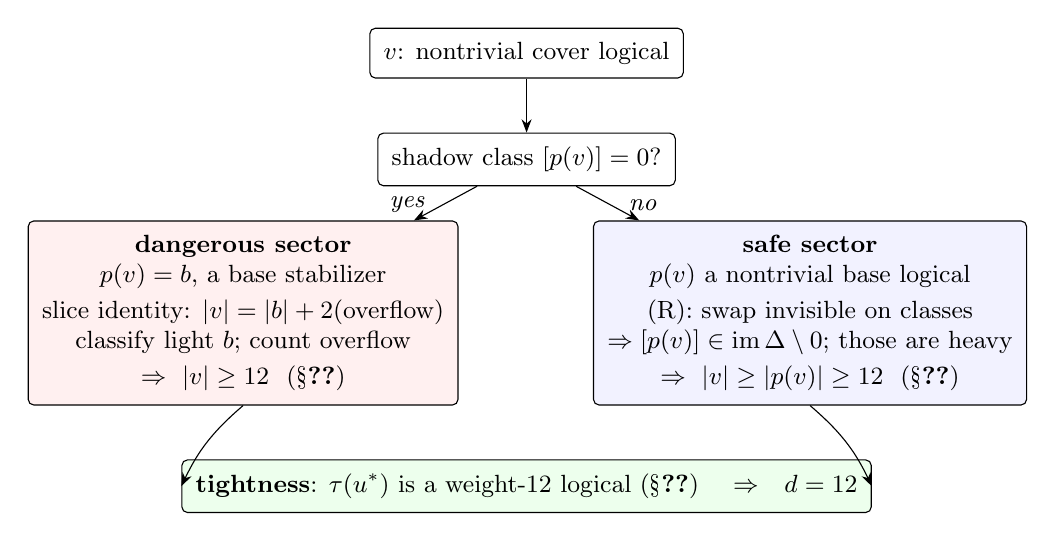
\begin{tikzpicture}[
  box/.style={draw, rounded corners=2pt, align=center, inner sep=5pt,
              font=\small},
  lab/.style={font=\small\itshape},
  >={Stealth}]
\node[box] (v) at (0,0) {$v$: nontrivial cover logical};
\node[box] (q) at (0,-1.35) {shadow class $[p(v)] = 0$?};
\node[box, fill=red!6] (dang) at (-3.6,-3.3)
  {\textbf{dangerous sector}\\
   $p(v) = b$, a base stabilizer\\[2pt]
   slice identity: $\wt{v} = \wt{b} + 2(\text{overflow})$\\
   classify light $b$; count overflow\\[2pt]
   $\Rightarrow\ \wt{v} \geq 12$ \ (\S\ref{sec:dangerous})};
\node[box, fill=blue!5] (safe) at (3.6,-3.3)
  {\textbf{safe sector}\\
   $p(v)$ a nontrivial base logical\\[2pt]
   (R): swap invisible on classes\\
   $\Rightarrow [p(v)] \in \imD\setminus 0$; those are heavy\\[2pt]
   $\Rightarrow\ \wt{v} \geq \wt{p(v)} \geq 12$ \ (\S\ref{sec:safe})};
\node[box, fill=green!7] (tight) at (0,-5.5)
  {\textbf{tightness}: $\tau(u^*)$ is a weight-12 logical
   (\S\ref{sec:tightness}) \quad$\Rightarrow$\quad $d = 12$};
\draw[->] (v) -- (q);
\draw[->] (q) -- node[lab, pos=0.55, left=3pt]{yes} (dang);
\draw[->] (q) -- node[lab, pos=0.55, right=3pt]{no} (safe);
\draw[->] (dang.south) to[bend right=12] (tight.west);
\draw[->] (safe.south) to[bend left=12] (tight.east);
\end{tikzpicture}
\caption{The architecture. Both sectors are forced to weight $\geq 12$ by
different mechanisms; one explicit diagonal lift attains it.}
\label{fig:architecture}
\end{figure}

And here is the promised accounting of what must be \emph{known} to run the
argument --- note every item lives on the base side:

\begin{enumerate}[leftmargin=2.4em,label=\textbf{I\arabic*.}]
\item \textbf{(T-A)} No nonzero base cycle of weight $\leq 5$
  (Section~\ref{sec:warmup}); plus the explicit weight-6 logical $u^*$.
\item \textbf{(CLASS)} A classification of the base's \emph{light
  stabilizers}: every nonzero stabilizer of weight $\leq 11$ is one of two
  explicit families (Section~\ref{sec:dangerous}).
\item \textbf{(R)} A single polynomial identity in $\Rcov$ certifying that the
  swap acts trivially on cover classes (Section~\ref{sec:safe}).
\item \textbf{(M-im)} The \emph{heavy classes} statement: every base cycle
  whose class lies in $\imD \setminus 0$ has weight $\geq 12$
  (Section~\ref{sec:safe}).
\item \textbf{(WIT)} The witness certificate: $[u^*] \notin \imD$
  (Section~\ref{sec:tightness}).
\end{enumerate}

I1 and the two flagged black boxes (I2, I4) are finite statements about the
72-qubit code. I3 is one line of polynomial algebra. I5 is one evaluation of
an explicit linear functional. That is the entire bill of materials for
$d(\mathrm{gross}) = 12$.

% ==================================================================
\section{The dangerous sector}
\label{sec:dangerous}
% ==================================================================

In this sector the fold is useless as a weight bound: the shadow of a
dangerous logical is a stabilizer, possibly light, possibly zero, so
$\wt{v} \geq \wt{p(v)}$ tells us little or nothing. We therefore change
instruments. Instead of projecting $v$ and weighing the result, we compare
its two sheets \emph{with each other} --- profitable because dangerous
logicals are, structurally, \emph{almost diagonal}.

Here is that structure. Throughout this section $v$ is a nontrivial
dangerous logical: $[p(v)] = 0$. By the fold criterion
(Proposition~\ref{prop:fold}),
\[
v = \tau(u) + \widetilde S(\widetilde z), \qquad u \text{ a base cycle with }
[u] \notin \imD .
\]
Fold the parametrization: the diagonal lift contributes nothing, and
$p \circ \widetilde S = S \circ p$ (Lemma~\ref{lem:transport}(1)), so the
shadow
\[
b \;:=\; p(v) \;=\; S(p(\widetilde z))
\]
is a base \emph{stabilizer}; and since $p(v) = v_0 + v_1$, the sheets
satisfy $v_1 = v_0 + b$ --- \emph{the two sheets agree everywhere except on
the shadow's support}. We must show $\wt{v} \geq 12$, whatever $b$ is. The
plan: an exact identity expressing $\wt{v}$ through $b$ and a ``sheet
overflow'' term (\S\ref{sec:dangerous}.1); a classification of the possible
light $b$ (\S\ref{sec:dangerous}.3); and a counting argument for each class
(\S\ref{sec:dangerous}.4).

\subsection{The slice identity}

\begin{lemma}[slice identity]\label{lem:slice}
Let $v$ be any cover operator with sheets $(v_0, v_1)$ and shadow $b = v_0 +
v_1$. Then
\[
\wt{v} \;=\; \wt{b} \;+\; 2\,\wt{v_0 \text{ off } \suppop b}.
\]
\end{lemma}

\begin{proof}
Count cell by cell over the base grid. Over a cell in $\suppop b$: the two
sheet values differ (their sum is 1), so exactly one of the two cover cells is
occupied --- contributing $\wt{b}$ in total. Over a cell outside $\suppop b$:
the sheet values agree, contributing $0$ or $2$; the $2$'s happen exactly on
the support of $v_0$ off $\suppop b$ (equivalently $v_1$; they agree there).
\end{proof}

In words: over the shadow's support, $v$ pays exactly $\wt b$; everywhere
else, whatever sheet 0 does, sheet 1 must copy, at double cost. Note the
reading of the second term (the convention of Section~\ref{sec:setup}):
$\wt{v_0 \text{ off } \suppop b} = \lvert \suppop v_0 \setminus \suppop b
\rvert$ counts the \emph{qubits where the sheet acts but the shadow does
not} --- exactly the qubits occupied in both sheets, each charged twice.
This ``overflow'' is what we must bound below: if the shadow is light, the
sheets are nearly equal and near-diagonal weight-doubling should kick in. Formally, for each stabilizer $b$ define
\[
m(b) \;:=\; \min \bigl\{\, \wt{v_0 \text{ off } \suppop b} \;:\; v \text{ a
nontrivial dangerous logical with } p(v) = b \,\bigr\},
\]
so that every dangerous logical over $b$ has $\wt{v} \geq \wt{b} + 2m(b)$.
(Two sanity notes on the definition. Off $\suppop b$ the two sheets agree,
so the overflow is the same whichever sheet we read --- nothing depends on
the arbitrary labeling of sheet $0$. And if no dangerous logical at all has
shadow $b$, the minimum runs over the empty set and the rung below holds
vacuously.) The dangerous floor we are after reads:
\begin{equation}\label{eq:M}
\textbf{(M)}\qquad \wt{b} + 2\,m(b) \;\geq\; 12
\qquad\text{for every base stabilizer } b .
\end{equation}

\subsection{The easy rungs: \texorpdfstring{$b = 0$}{b=0} and heavy
\texorpdfstring{$b$}{b}}

\emph{Rung $b = 0$.} Then $v$ is diagonal: $v = \tau(u)$ with $[u] \notin
\imD$; in particular $u \neq 0$, so $\wt{u} \geq 6$ by (T-A) and $\wt{v} =
2\wt{u} \geq 12$. (This is the warm-up's Case 2, upgraded with the lift
criterion: nontriviality of $v$ needs $[u]\notin\imD$, and that is all it
needs.)

\emph{Rung $\wt{b} \geq 12$.} Immediate: $\wt{v} \geq \wt{b} \geq 12$, by the
slice identity or just Lemma~\ref{lem:transport}(2).

Everything now hinges on stabilizers of intermediate weight $1,\dots,11$. Two
cheap parity facts first. The \emph{augmentation} $\varepsilon : \F_2[G] \to
\F_2$ is evaluation at $x = y = 1$ --- a ring homomorphism, being an
evaluation --- and evaluating a polynomial with $0/1$ coefficients at $1$
just counts its terms mod 2: $\varepsilon(f) \equiv \wt{f} \pmod 2$. Since
$A$ and $B$ have three terms each, $\varepsilon(A) = \varepsilon(B) = 1$,
so multiplication by either preserves weight parity:
$\wt{Af} \equiv \varepsilon(Af) = \varepsilon(A)\,\varepsilon(f) =
\varepsilon(f) \equiv \wt{f} \pmod 2$. In particular every stabilizer has
even weight:
\[
\wt{S(z)} = \wt{Bz} + \wt{Az} \equiv \wt{z} + \wt{z} \equiv 0 \pmod 2 .
\]
So only $\wt{b} \in \{2,4,6,8,10\}$ can occur strictly between the rungs.

\subsection{Input 2: the light-stabilizer classification}

Which stabilizers of weight $\leq 11$ actually exist? Two families are easy to
write down.

\begin{definition}\label{def:hexdpair}
A \emph{hexagon} is a single $Z$-check, viewed as a stabilizer:
$S(\delta_g) = (B\delta_g,\, A\delta_g)$, the weight-6 pattern of
Section~\ref{sec:setup} stamped at $g$, with three cells in each block; write
$h(g)$ for its 6-cell support. A \emph{D-pair} is $S(\delta_g + \delta_h)$
with $g - h \in dA \cup dB$ (``D'' for \emph{difference}: the two generating
cells are offset by an element of the difference sets of
Definition~\ref{def:diffsets}). Its weight is exactly $10$: on one block the two translates
overlap in exactly one cell (multiplicity-freeness of the difference sets) and
cancel there --- $Z \cdot Z = I$ on the shared qubit --- giving
$3 + 3 - 2 = 4$; on the other block $g - h$ avoids the
other difference set (disjointness!), giving $6$. The union of the two
hexagons has $11$ cells: the $10$ of $\suppop b$ plus the one cancelled cell,
which we call $q^*$.
\end{definition}

\begin{figure}[ht]
\centering
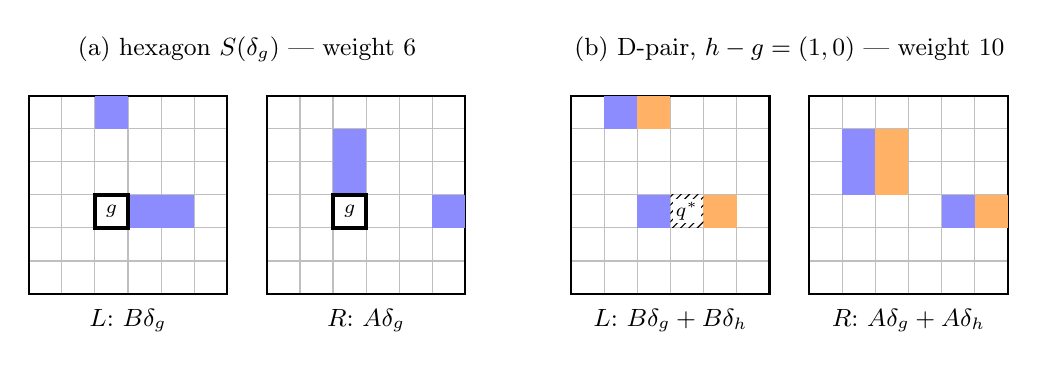
\begin{tikzpicture}[scale=0.42]
% ----- panel (a): hexagon at g=(2,2) -----
\node at (6.6,7.4) {\small (a)\ hexagon $S(\delta_g)$ --- weight $6$};
\begin{scope}
\draw[step=1,gray!50,thin] (0,0) grid (6,6);
\draw[thick] (0,0) rectangle (6,6);
\node[anchor=north] at (3,-0.15) {\small $L$:\ $B\delta_g$};
\fill[blue!45] (2,5) rectangle +(1,1);
\fill[blue!45] (3,2) rectangle +(1,1);
\fill[blue!45] (4,2) rectangle +(1,1);
\draw[very thick] (2,2) rectangle +(1,1);
\node at (2.5,2.5) {\scriptsize $g$};
\end{scope}
\begin{scope}[shift={(7.2,0)}]
\draw[step=1,gray!50,thin] (0,0) grid (6,6);
\draw[thick] (0,0) rectangle (6,6);
\node[anchor=north] at (3,-0.15) {\small $R$:\ $A\delta_g$};
\fill[blue!45] (5,2) rectangle +(1,1);
\fill[blue!45] (2,3) rectangle +(1,1);
\fill[blue!45] (2,4) rectangle +(1,1);
\draw[very thick] (2,2) rectangle +(1,1);
\node at (2.5,2.5) {\scriptsize $g$};
\end{scope}
% ----- panel (b): D-pair, g=(1,2), h=(2,2), offset (1,0) in dB -----
\node at (23,7.4) {\small (b)\ D-pair, $h - g = (1,0)$ --- weight $10$};
\begin{scope}[shift={(16.4,0)}]
\draw[step=1,gray!50,thin] (0,0) grid (6,6);
\draw[thick] (0,0) rectangle (6,6);
\node[anchor=north] at (3,-0.15) {\small $L$:\ $B\delta_g + B\delta_h$};
\fill[blue!45] (1,5) rectangle +(1,1);
\fill[blue!45] (2,2) rectangle +(1,1);
\fill[orange!60] (2,5) rectangle +(1,1);
\fill[orange!60] (4,2) rectangle +(1,1);
\fill[pattern=north east lines] (3,2) rectangle +(1,1);
\node[fill=white, inner sep=1pt] at (3.5,2.5) {\scriptsize $q^{*}$};
\end{scope}
\begin{scope}[shift={(23.6,0)}]
\draw[step=1,gray!50,thin] (0,0) grid (6,6);
\draw[thick] (0,0) rectangle (6,6);
\node[anchor=north] at (3,-0.15) {\small $R$:\ $A\delta_g + A\delta_h$};
\fill[blue!45] (4,2) rectangle +(1,1);
\fill[blue!45] (1,3) rectangle +(1,1);
\fill[blue!45] (1,4) rectangle +(1,1);
\fill[orange!60] (5,2) rectangle +(1,1);
\fill[orange!60] (2,3) rectangle +(1,1);
\fill[orange!60] (2,4) rectangle +(1,1);
\end{scope}
\end{tikzpicture}
\caption{The two light-stabilizer families, drawn on the base grids (one
$6\times 6$ grid per qubit block). (a) A single $Z$-check: the pattern
$(B\delta_g, A\delta_g)$ stamped at the outlined cell $g = (2,2)$. (b) The product
of the checks at $g$ (blue) and $h = g + (1,0)$ (orange): on the $L$ block
the two $B$-translates overlap in the hatched cell $q^*$, where
$Z \cdot Z = I$ cancels, leaving $3 + 3 - 2 = 4$ cells; on the $R$ block
the offset $(1,0) \notin dA$ forces no overlap, leaving $6$. Total weight
$10$; the $11$-cell union $U = \suppop b \cup \{q^*\}$ is the window of the
D-pair counting rung.}
\label{fig:hexdpair}
\end{figure}

Figure~\ref{fig:hexdpair} draws both objects. For gross's base there are
$36$ hexagons (one per cell) and $216$ D-pairs ($36$ choices of $g$, $12$
possible offsets, halved because $\{g,h\}$ is unordered). The hard theorem
--- our second black box --- is that there is nothing else:

\begin{inputbox}[Input (CLASS): light stabilizers are classified]
\textbf{Theorem} (program write-up, \S6.3; fully hand-proved). Every nonzero
stabilizer of the base code with weight $\leq 11$ is a hexagon or a D-pair. In
particular there are no stabilizers of weights $2, 4,$ or $8$, and the minimum
stabilizer weight is $6$.
\end{inputbox}

It is worth pausing on what kind of problem this is. In pictures: you hold
a two-board stencil --- $\suppop B$ for the $L$ board, $\suppop A$ for the
$R$ board --- and you may stamp it, in lockstep on both boards, at any set
of positions of the torus; stamps add mod 2. The stabilizer group is
everything you can produce, and the classification asks \emph{which
low-weight pictures are producible, and how}. Few stamps are controlled by
Definition~\ref{def:diffsets}: one stamp always weighs exactly $6$; two
stamps weigh $12 - 2(\text{overlaps})$, and multiplicity-freeness plus
disjointness cap the overlaps at one, so two stamps weigh $10$ or $12$.
The theorem's real content is about \emph{many} stamps: no orchestration
of dozens of stamps cancels below $12$, except the one- and two-stamp
patterns already listed. That is genuinely special to the code, not a
formality --- the $\Z_6 \times \Z_{14}$ cousin appearing in
Section~\ref{sec:window} has weight-$8$ pictures whose cheapest production
takes $36$ stamps. (At the extreme, the stamp-sets whose picture is
entirely \emph{blank} are exactly the relations $K$ of
Section~\ref{sec:lift}.) In classical terms this is the low-weight-codeword
problem for the linear code spanned by all translates of the double stencil
--- BB codes were in fact born as ``quasi-cyclic'' objects of classical
coding theory \cite{kovalevpryadko} --- but no off-the-shelf classical
theorem delivers the census: the named distance bounds for cyclic and
abelian codes see only the odd part of the group, and here the interesting
cancellations live in the $2$-part.

(How does one prove such a thing? By a finite case analysis on the ``layer
profile'' of the two blocks of $b = S(z)$, run in a Fourier-like coordinate
system adapted to $\Z_6^2 \cong \Z_2^2 \times \Z_3^2$ --- the natural tool,
since stamping is translation-invariant and Fourier diagonalizes
translation; each case is a few lines, and the whole analysis is a couple
of pages. Nothing about it is deep, but it is genuinely code-specific ---
it consumes the exact shape of $A$ and $B$. This is where the polynomials
earn their keep.)

\subsection{The counting rungs: hexagons and D-pairs}

Two rungs remain:
\[
m(\text{hexagon}) \geq 3
\qquad\text{and}\qquad
m(\text{D-pair}) \geq 1 ,
\]
which deliver $6 + 2 \cdot 3 \geq 12$ and $10 + 2 \cdot 1 \geq 12$. Both
run on one intuition: \emph{a nontrivial cycle cannot hide in a small
window}. If the overflow were too small, the sheet $v_0$ would be --- up
to corrections we can control --- a cycle of nontrivial class crammed into
a $6$- or $11$-cell window; (T-A) forbids nonzero cycles of weight
$\leq 5$, and class-nontriviality blocks the escape route of being zero.
The counting below makes ``crammed'' quantitative.

The phrase ``corrections we can control'' is the content of the next
lemma. The point to hold on to: the parametrization
$v = \tau(u) + \widetilde S(\widetilde z)$ of a dangerous logical is far
from unique, and the proof \emph{spends that freedom}. It standardizes the
stabilizer term in two moves, each of which transfers a diagonal summand
out of the stabilizer term and into the $\tau(u)$ term. The transfers are
harmless because the class of $u$ only ever shifts by elements of $\imD$
--- and ``outside $\imD$'' survives such shifts. Once the stabilizer term
is fully standardized, its sheet can be read off by eye: it is trapped in
the window drawn in Figure~\ref{fig:hexdpair}.

\begin{lemma}[carry support]\label{lem:carrysupport}
Let $v$ be a nontrivial dangerous logical with shadow $b$. Then its sheet can
be written
\[
v_0 \;=\; u' + c,
\]
where $u'$ is a base cycle with $[u'] \notin \imD$, and $c$ is a ``carry''
vector with
\[
\suppop c \subseteq \suppop b \quad (b \text{ a hexagon}), \qquad
\suppop c \subseteq \suppop b \cup \{q^*\} \quad (b \text{ a D-pair}).
\]
\end{lemma}

\begin{proof}
Write $v = \tau(u) + \widetilde S(\widetilde z)$ with $[u] \notin \imD$
(fold criterion), and let $z := p(\widetilde z)$, so $S(z) = b$. The plan:
two standardizing moves, then a read-off.

\emph{Move 1: standardize the lift.} The cover element $\widetilde z$
differs from the exponent-restricted lift of $z$ by an element of
$\ker p$: $\widetilde z = \widetilde{z}^{\,\mathrm{res}} +
(1+x^6)\,\widetilde r$ (Lemma~\ref{lem:diagonal}). Applying $\widetilde S$
and using the master identity~\eqref{eq:master} together with
$p \circ \widetilde S = S \circ p$,
\[
\widetilde S(\widetilde z) = \widetilde S(\widetilde z^{\,\mathrm{res}})
+ (1+x^6)\,\widetilde S(\widetilde r)
= \widetilde S(\widetilde z^{\,\mathrm{res}}) +
\tau\bigl(S(p(\widetilde r))\bigr).
\]
The last summand is the diagonal lift of a base \emph{stabilizer}:
transfer it into the $\tau(u)$ term, replacing $u$ by
$u + S(p(\widetilde r))$. The class $[u]$ is unchanged.

\emph{Move 2: standardize the preimage.} Preimages of $b$ under $S$ differ
by elements of $\ker S = K$: $z = z_b + \kappa$ with $z_b$ our favourite
preimage ($\delta_g$ for a hexagon, $\delta_g + \delta_h$ for a D-pair)
and $\kappa \in K$. Lifting is linear, so
$\widetilde S(\widetilde z^{\,\mathrm{res}}) =
\widetilde S(\widetilde{z_b}) + \widetilde S(\widetilde\kappa)$, and by
the seam-carry lemma (Lemma~\ref{lem:seamcarry}) the second summand is
$\tau(\Delta\kappa)$ --- diagonal again. Transfer it too, replacing $u$ by
$u + \Delta\kappa$: this time the class does shift, but only \emph{by} an
element of $\imD$, and ``outside $\imD$'' is stable under such shifts.
Call the final result $u'$.

\emph{Read-off.} We now have $v = \tau(u') + \widetilde S(\widetilde{z_b})$
with $[u'] \notin \imD$; set $c := \text{sheet 0 of }\widetilde
S(\widetilde{z_b})$, so that $v_0 = u' + c$. Where can $c$ live? Every
occupied cover cell of $\widetilde S(\widetilde{z_b})$ lies over the
support of one of the constituent checks. For the hexagon (one check),
those six cover cells all lie over $h(g) = \suppop b$, whichever sheet
each lands in. For the D-pair (two checks), the at most twelve occupied
cover cells lie over the union of the two hexagons --- the blue, orange,
and hatched cells of Figure~\ref{fig:hexdpair}(b) --- which is
$\suppop b \cup \{q^*\}$: everything sits over the shadow's support except
possibly the two cover cells over the cancelled cell $q^*$, which
cancelled downstairs but may sit in \emph{different sheets} upstairs and
survive. (Cancellation downstairs can fail upstairs: the seam again.)
Reading off sheet $0$: $\suppop c \subseteq \suppop b$, respectively
$\suppop c \subseteq \suppop b \cup \{q^*\}$, as claimed.
\end{proof}

\begin{figure}[ht]
\centering
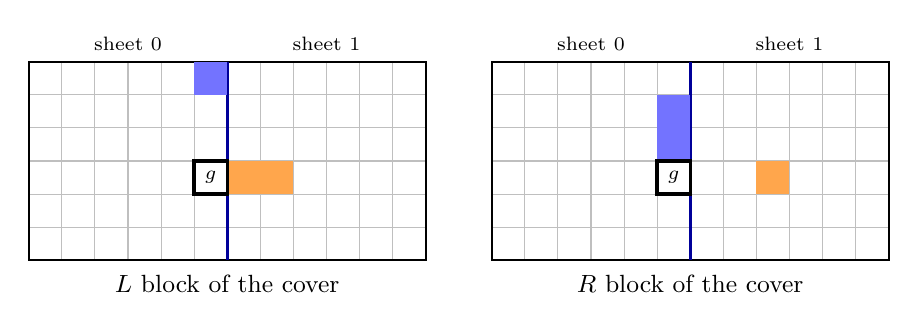
\begin{tikzpicture}[scale=0.42]
% L cover block
\begin{scope}
\draw[step=1,gray!50,thin] (0,0) grid (12,6);
\draw[thick] (0,0) rectangle (12,6);
\draw[very thick,blue!60!black] (6,0) -- (6,6);
\node[anchor=north] at (6,-0.15) {\small $L$ block of the cover};
\fill[blue!55] (5,5) rectangle +(1,1);
\fill[orange!70] (6,2) rectangle +(1,1);
\fill[orange!70] (7,2) rectangle +(1,1);
\draw[very thick] (5,2) rectangle +(1,1);
\node at (5.5,2.5) {\scriptsize $g$};
\node[anchor=south] at (3,6.05) {\scriptsize sheet $0$};
\node[anchor=south] at (9,6.05) {\scriptsize sheet $1$};
\end{scope}
% R cover block
\begin{scope}[shift={(14,0)}]
\draw[step=1,gray!50,thin] (0,0) grid (12,6);
\draw[thick] (0,0) rectangle (12,6);
\draw[very thick,blue!60!black] (6,0) -- (6,6);
\node[anchor=north] at (6,-0.15) {\small $R$ block of the cover};
\fill[blue!55] (5,3) rectangle +(1,1);
\fill[blue!55] (5,4) rectangle +(1,1);
\fill[orange!70] (8,2) rectangle +(1,1);
\draw[very thick] (5,2) rectangle +(1,1);
\node at (5.5,2.5) {\scriptsize $g$};
\node[anchor=south] at (3,6.05) {\scriptsize sheet $0$};
\node[anchor=south] at (9,6.05) {\scriptsize sheet $1$};
\end{scope}
\end{tikzpicture}
\caption{The carry, concretely (Example~\ref{ex:carry}): the check stamped
at $g = (5,2)$ straddles the seam. Of its six cover cells, three (blue)
land in sheet $0$ --- they form the carry $c$ --- and three (orange) land
in sheet $1$; folding either trio lands inside $\suppop b$. A stamp that
stays clear of the seam, like $g = (2,2)$ in Figure~\ref{fig:hexdpair}(a),
puts all six cells in one sheet, and $c$ is the whole of $\suppop b$.}
\label{fig:carry}
\end{figure}

\begin{example}[the carry, concretely]\label{ex:carry}
Stamp the check at $g = (5,2)$ --- chosen deliberately so the stamp
straddles the seam --- and trace the read-off (Figure~\ref{fig:carry}).
Upstairs, $\widetilde S(\widetilde\delta_g)$ occupies six cover cells: on
the $L$ block, $(5,5)$, $(6,2)$, $(7,2)$; on the $R$ block, $(8,2)$,
$(5,3)$, $(5,4)$. Three have $x$-coordinate below $6$ (sheet $0$) and
three have $x$-coordinate $6, 7, 8$ (sheet $1$). So the sheets of
$\widetilde S(\widetilde\delta_g)$ are $(c,\ b + c)$ with
\[
c \;=\; \bigl(\text{$L$: } (5,5);\quad \text{$R$: } (5,3),\, (5,4)\bigr),
\]
and folding confirms $\suppop c \subseteq \suppop b$. A dangerous logical
over this $b$ therefore has sheets $v_0 = u' + c$ and $v_1 = u' + c + b$.
For contrast, the stamp at $g = (2,2)$ of Figure~\ref{fig:hexdpair}(a)
stays clear of the seam: all six cover cells sit in sheet $0$, so there
$c$ is the \emph{whole} of $\suppop b$ and sheet $1$ receives nothing.
Either way --- and this is the lemma's point --- the carry never escapes
the window.
\end{example}

\begin{theorem}[counting rungs]\label{thm:rungs}
$m(\text{hexagon}) \geq 3$ and $m(\text{D-pair}) \geq 1$.
\end{theorem}

\begin{proof}
\emph{Hexagons.} Let $b$ be a hexagon with support $h$, $\wt{b} = 6$. By
Lemma~\ref{lem:carrysupport}, $v_0 = u' + c$ with $\suppop c \subseteq h$,
so off $h$ the sheet and $u'$ agree, and the overflow equals
$\wt{u' \text{ off } h}$. It therefore suffices to show that \emph{every}
base cycle $u'$ with $[u'] \notin \imD$ has $\wt{u' \text{ off } h} \geq
3$.

Suppose not: $\wt{u' \text{ off } h} \leq 2$. Play $u'$ against its
partner $u' + b$. The two agree off $h$ (as $\suppop b = h$), and at each
cell of $h$ exactly one of them is occupied ($b$ equals $1$ there), so the
six cells of $h$ split between them:
\[
\wt{u' \cap h} \;+\; \wt{(u'+b) \cap h} \;=\; 6 .
\]
One of the two --- call it $w$ --- therefore has at most $3$ cells on $h$,
hence $\wt{w} \leq 3 + 2 = 5$ in total. But $[w] = [u'] \notin \imD$
(adding the stabilizer $b$ does not move the class); in particular
$[w] \neq 0$, since the zero class lies in $\imD$, so $w \neq 0$. A
nonzero cycle of weight $\leq 5$ contradicts (T-A).

\emph{D-pairs.} Let $b = b_1 + b_2$ with constituent hexagons
$b_1 = S(\delta_g)$, $b_2 = S(\delta_h)$, and window
$U := \suppop b \cup \{q^*\}$, $|U| = 11$
(Figure~\ref{fig:hexdpair}(b)). By Lemma~\ref{lem:carrysupport},
$v_0 = u' + c$ with $\suppop c \subseteq U$. Suppose the overflow were
$0$. Then $u' + c$ vanishes off $\suppop b$, hence certainly off the
larger set $U$; and off $U$ the carry $c$ is itself zero, so $u'$ vanishes
off $U$: a nontrivial cycle crammed into eleven cells. We rule this out by
averaging over the four ways of adding the constituent hexagons. Consider
\[
u',\qquad u' + b_1,\qquad u' + b_2,\qquad u' + b_1 + b_2 ,
\]
and count their total weight twice.
\begin{itemize}[leftmargin=2em]
\item \emph{From below.} Each of the four has class $[u'] \notin \imD$,
  hence is nonzero, hence weighs $\geq 6$ by (T-A). Total: $\geq 24$.
\item \emph{Exactly, cell by cell.} All four are supported inside $U$
  ($u'$ is, and so are $b_1$ and $b_2$). At a cell $q \in U$, at least
  one of $b_1(q), b_2(q)$ equals $1$ --- that is what $q \in U$ means ---
  so the four added offsets $0,\ b_1(q),\ b_2(q),\ b_1(q){+}b_2(q)$
  always comprise two $0$'s and two $1$'s. Adding the common value
  $u'(q)$ preserves the two--two split, so \emph{exactly two} of the four
  cycles occupy $q$, whatever $u'$ does. Total: exactly $2|U| = 22$.
\end{itemize}
Together, $24 \leq 22$ --- a contradiction. Hence the overflow is
$\geq 1$.
\end{proof}

\begin{figure}[ht]
\centering
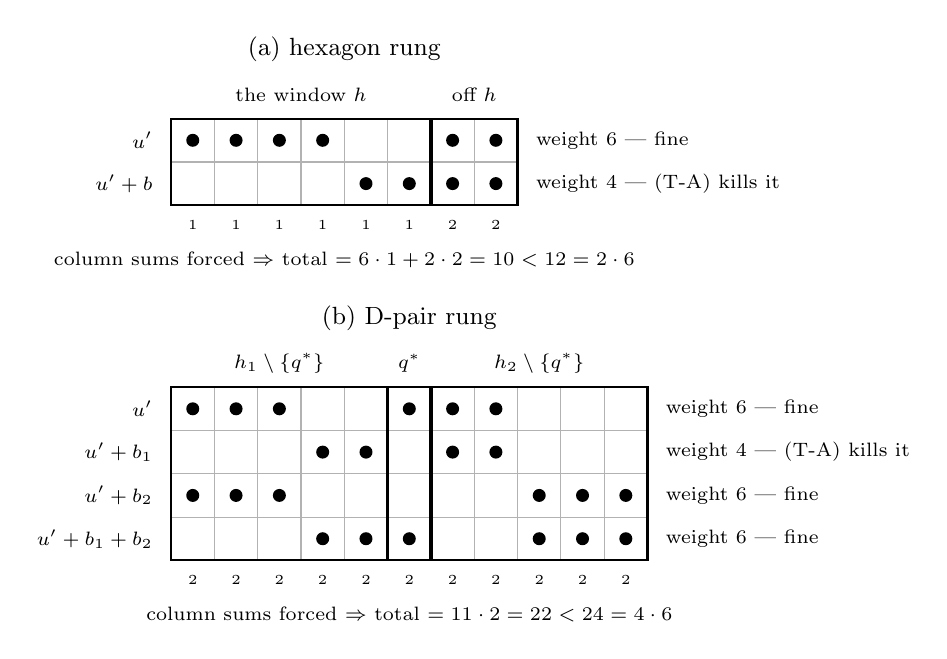
\begin{tikzpicture}[xscale=0.55,yscale=0.55]
% ---------- panel (a): hexagon, 2 x 8 ----------
\begin{scope}
\node at (4,3.6) {\small (a) hexagon rung};
\node at (3,2.55) {\scriptsize the window $h$};
\node at (7,2.55) {\scriptsize off $h$};
\draw[step=1,gray!60,thin] (0,0) grid (8,2);
\draw[thick] (0,0) rectangle (8,2);
\draw[very thick] (6,0) -- (6,2);
\foreach \c in {0,1,2,3,6,7} {\fill (\c+0.5,1.5) circle (0.15);}
\foreach \c in {4,5,6,7} {\fill (\c+0.5,0.5) circle (0.15);}
\node[anchor=east] at (-0.2,1.5) {\scriptsize $u'$};
\node[anchor=east] at (-0.2,0.5) {\scriptsize $u'+b$};
\node[anchor=west] at (8.2,1.5) {\scriptsize weight $6$ --- fine};
\node[anchor=west] at (8.2,0.5) {\scriptsize weight $4$ --- (T-A) kills it};
\foreach \c in {0,...,5} {\node at (\c+0.5,-0.45) {\tiny $1$};}
\foreach \c in {6,7} {\node at (\c+0.5,-0.45) {\tiny $2$};}
\node[anchor=north] at (4,-0.85)
  {\scriptsize column sums forced $\Rightarrow$ total
   $= 6 \cdot 1 + 2 \cdot 2 = 10 < 12 = 2 \cdot 6$};
\end{scope}
% ---------- panel (b): D-pair, 4 x 11 ----------
\begin{scope}[shift={(0,-8.2)}]
\node at (5.5,5.6) {\small (b) D-pair rung};
\node at (2.5,4.55) {\scriptsize $h_1 \setminus \{q^*\}$};
\node at (5.5,4.55) {\scriptsize $q^*$};
\node at (8.5,4.55) {\scriptsize $h_2 \setminus \{q^*\}$};
\draw[step=1,gray!60,thin] (0,0) grid (11,4);
\draw[thick] (0,0) rectangle (11,4);
\draw[very thick] (5,0) -- (5,4);
\draw[very thick] (6,0) -- (6,4);
\foreach \c in {0,1,2,5,6,7} {\fill (\c+0.5,3.5) circle (0.15);}
\foreach \c in {3,4,6,7} {\fill (\c+0.5,2.5) circle (0.15);}
\foreach \c in {0,1,2,8,9,10} {\fill (\c+0.5,1.5) circle (0.15);}
\foreach \c in {3,4,5,8,9,10} {\fill (\c+0.5,0.5) circle (0.15);}
\node[anchor=east] at (-0.2,3.5) {\scriptsize $u'$};
\node[anchor=east] at (-0.2,2.5) {\scriptsize $u'+b_1$};
\node[anchor=east] at (-0.2,1.5) {\scriptsize $u'+b_2$};
\node[anchor=east] at (-0.2,0.5) {\scriptsize $u'+b_1+b_2$};
\node[anchor=west] at (11.2,3.5) {\scriptsize weight $6$ --- fine};
\node[anchor=west] at (11.2,2.5) {\scriptsize weight $4$ --- (T-A) kills it};
\node[anchor=west] at (11.2,1.5) {\scriptsize weight $6$ --- fine};
\node[anchor=west] at (11.2,0.5) {\scriptsize weight $6$ --- fine};
\foreach \c in {0,...,10} {\node at (\c+0.5,-0.45) {\tiny $2$};}
\node[anchor=north] at (5.5,-0.85)
  {\scriptsize column sums forced $\Rightarrow$ total
   $= 11 \cdot 2 = 22 < 24 = 4 \cdot 6$};
\end{scope}
\end{tikzpicture}
\caption{The two counting rungs as \emph{occupancy matrices}
(Example~\ref{ex:counts}): one row per cycle, one column per cell, a dot
where the cycle occupies the cell. Row sums are weights, and (T-A) demands
every row reach $6$; but the column sums are \emph{forced} ($1$ per window
cell in (a), $2$ per cell in (b), doubled off-window in (a)), so the grand
total is too small for all rows to comply. Some row must dip --- here the
$u' + b$ rows --- and (T-A) kills it.}
\label{fig:matrices}
\end{figure}

\begin{example}[watching the counts kill a candidate]\label{ex:counts}
The two proofs are contradiction machines; here is each machine running on
a concrete victim, drawn in Figure~\ref{fig:matrices}.

\emph{Hexagon.} Suppose a dangerous logical over a hexagon $b$ had
overflow $2$: its $u'$ occupies four cells of the window $h$ and two cells
outside. On its own, $u'$ is unimpeachable --- weight $6$, no quarrel with
(T-A). But the partner $u' + b$ is forced to occupy exactly the
\emph{other two} cells of $h$ (each $h$-column of the matrix carries
exactly one dot, because $b$ is $1$ there) together with the same two
outside cells: weight $4$. Same class, weight below $6$ --- (T-A) kills
the partner, and the candidate dies with it.

\emph{D-pair.} Suppose a dangerous logical over a D-pair had overflow $0$,
so $u'$ is crammed into the eleven-cell window $U$: say three cells of
$h_1 \setminus \{q^*\}$, the overlap cell $q^*$, and two cells of
$h_2 \setminus \{q^*\}$ --- again weight $6$, again unimpeachable alone.
Now every column of the four-row matrix carries exactly two dots, so the
dots total $2 \cdot 11 = 22$, while four (T-A)-compliant rows would need
$24$. Some row must fall short --- in this instance $u' + b_1$, at weight
$4$ --- and (T-A) kills it.

The particular candidates are illustrative, not special: \emph{whatever}
$u'$ does, the column sums are forced, so the total is too small for every
row to clear (T-A). That forced shortfall is the entire content of both
rungs --- and Section~\ref{sec:window} runs the same machine at every
size, with $2^r$ rows and column sums $2^{r-1}$.
\end{example}

\subsection{The dangerous floor}

Assemble the rungs. For a nontrivial dangerous logical $v$ with shadow $b$:

\begin{center}
\begin{tabular}{lll}
\toprule
$b$ & bound used & $\wt{b} + 2m(b) \geq$\\
\midrule
$0$ & $m \geq 6$ \ (T-A on the diagonal half) & $12$\\
hexagon ($\wt b = 6$) & $m \geq 3$ \ (Theorem~\ref{thm:rungs}) & $12$\\
D-pair ($\wt b = 10$) & $m \geq 1$ \ (Theorem~\ref{thm:rungs}) & $12$\\
other, $0 < \wt b \leq 11$ & none exist \ (CLASS) & ---\\
$\wt b \geq 12$ & trivial & $12$\\
\bottomrule
\end{tabular}
\end{center}

\begin{theorem}[dangerous floor]\label{thm:dangerous}
Every nontrivial dangerous logical of the cover has weight $\geq 12$.
\end{theorem}

Notice the eerie precision: all three nontrivial rungs land \emph{exactly} on
$12$. The bound is genuinely tight on the $b = 0$ rung --- diagonal lifts of
weight-6 base logicals, which Section~\ref{sec:tightness} will certify --- and
only there: a finer analysis in the program's write-up shows the true minimum
over dangerous logicals with $b \neq 0$ is $14$.

\subsection{Second look: one lemma behind both rungs}
\label{sec:window}

The two counting arguments just given are suspiciously similar --- a
pigeonhole over two cycles, an average over four --- and the resemblance is
not a coincidence. They are the same computation run at different sizes,
and exhibiting the general statement pays twice: it packages the entire
dangerous floor into three checkable hypotheses, and it shows exactly what
the classification (CLASS) is \emph{for}.

\begin{definition}[windowed decomposition]
Let $b \neq 0$ be a base stabilizer. A \emph{windowed decomposition} of $b$
is a choice of preimage: a set of $r$ cells, recorded as $z_b \in \F_2[G]$
with $S(z_b) = b$, expressing $b$ as the product of the $r$ checks at those
cells. Its \emph{window} is the union of those checks' supports,
\[
U \;=\; \bigcup_{g \,\in\, \suppop z_b} h(g) ,
\]
so $\suppop b \subseteq U$, with equality exactly when nothing cancelled.
(Hexagons: $r = 1$, $U = \suppop b$. D-pairs: $r = 2$, $U = \suppop b \cup
\{q^*\}$.)
\end{definition}

\begin{lemma}[window averaging]\label{lem:window}
Let $d$ be a \emph{cycle floor} for the base (every nonzero base cycle,
stabilizers included, has weight $\geq d$), and let $b \neq 0$ admit a
windowed decomposition with window $U$. Then
\[
m(b) \;\geq\; \Bigl\lceil\, d - \tfrac{|U|}{2} \,\Bigr\rceil ,
\]
so every nontrivial dangerous logical $v$ with $p(v) = b$ has
$\wt{v} \geq \wt{b} + 2\lceil d - |U|/2 \rceil$.
\end{lemma}

\begin{proof}
The carry-support lemma runs verbatim with this $z_b$: its two
standardizing moves never used the shape of $z_b$, and in the read-off
every occupied cover cell of $\widetilde S(\widetilde{z_b})$ lies over the
support of one of the $r$ constituent checks, i.e.\ over $U$. So $v_0 = u' + c$ with
$[u'] \notin \imD$ and $\suppop c \subseteq U$, and the overflow is at
least $e := \wt{u' \text{ off } U}$.

Now average. For each of the $2^r$ subsets $T$ of the $r$ check positions,
\[
u'_T \;:=\; u' + \textstyle\sum_{g \in T} S(\delta_g)
\]
is a cycle of class $[u'] \notin \imD$, hence nonzero, hence of weight
$\geq d$: total weight $\geq 2^r d$. Count the same total cell by cell.
Off $U$ every $u'_T$ agrees with $u'$: contribution $2^r e$. At a cell
$q \in U$, the map $T \mapsto \sum_{g \in T} S(\delta_g)(q)$ is a
\emph{nonzero} $\F_2$-linear functional of the indicator of $T$ (nonzero
because some check covers $q$ --- that is what $q \in U$ means), so it
takes each value on exactly $2^{r-1}$ subsets; adding the constant
$u'(q)$ does not change the count, so exactly $2^{r-1}$ of the $u'_T$
occupy $q$. Contribution: exactly $2^{r-1}|U|$. Hence
\[
2^r d \;\leq\; 2^{r-1}|U| + 2^r e
\qquad\Longrightarrow\qquad
e \;\geq\; d - \tfrac{|U|}{2},
\]
and $e$ is an integer, so the ceiling holds. Finish with the slice
identity.
\end{proof}

Check it against Section~\ref{sec:dangerous}.4: the hexagon rung is
$r = 1$, $|U| = 6$, giving $m \geq \lceil 6 - 3 \rceil = 3$; the D-pair
rung is $r = 2$, $|U| = 11$, giving $m \geq \lceil 6 - 5.5 \rceil = 1$.
The pigeonhole and the four-cycle average were one computation in two
disguises.

\begin{theorem}[generic dangerous floor]\label{thm:genericfloor}
For a doubling pair as in Section~\ref{sec:cover} (any
$\Z_\ell \times \Z_m$, same polynomials upstairs), suppose:
\begin{itemize}[leftmargin=3.2em]
\item[\textbf{(P)}] $\wt{A}$ and $\wt{B}$ are odd \hfill (parity)
\item[\textbf{(F)}] every nonzero base cycle has weight $\geq d$
  \hfill (cycle floor)
\item[\textbf{(W)}] every base stabilizer $b$ with
  $0 < \wt{b} \leq 2d - 2$ admits a windowed decomposition with
  $|U| \leq \wt{b} + 1$ \hfill (small windows)
\end{itemize}
Then every nontrivial dangerous logical of the cover has weight $\geq 2d$.
\end{theorem}

\begin{proof}
(P) gives $\varepsilon(A) = \varepsilon(B) = 1$, so stabilizer weights are
even (\S\ref{sec:dangerous}.2) and the possible shadows are $b = 0$, even
$\wt{b} \in [2,\, 2d{-}2]$, and $\wt{b} \geq 2d$. The first is the diagonal
rung: $v = \tau(u)$ with $[u] \notin \imD$, so $u \neq 0$ and (F) gives
$\wt{v} = 2\wt{u} \geq 2d$. The last is trivial. For the middle, (W) and
Lemma~\ref{lem:window} give
\[
\wt{v} \;\geq\; \wt{b} +
2\Bigl\lceil d - \tfrac{\wt{b}+1}{2} \Bigr\rceil
\;=\; \wt{b} + (2d - \wt{b}) \;=\; 2d ,
\]
the ceiling supplying the missing half because $2d - \wt{b}$ is even ---
parity again.
\end{proof}

Three remarks locate this statement in the landscape.

\begin{enumerate}[leftmargin=2.2em]
\item \emph{The classification's job is exactly hypothesis (W).} It
  enumerates the light stabilizers and either exhibits a tight
  decomposition for each family (hexagons: $|U| = \wt{b}$; D-pairs:
  $|U| = \wt{b} + 1$) or certifies that a weight is absent (no $2$, $4$,
  or $8$). That is the entire code-specific content of the dangerous half
  of the proof.
\item \emph{The hypotheses are sharp, with named exhibits.} (W) can fail
  even in an odd-weight code: the $\Z_6 \times \Z_{14}$ sibling code of
  Section~\ref{sec:instances} has a family of weight-8 stabilizers whose
  cheapest decomposition uses $36$ checks spanning a $110$-cell window
  (needed: $\leq 9$; the program's write-up states its missing rung in
  exactly this currency, ``needs $U \leq 9$''); no analytic rung is known
  for that family, and the instance survives only because it is far from
  binding. The parity scaffolding is load-bearing too: with $\wt{A},
  \wt{B}$ of \emph{opposite} parities, odd shadows appear and the same
  computation certifies only $2d - 1$; and dropping oddness altogether is
  fatal in the wild --- there is a weight-$4$-polynomial pair on
  $\Z_5 \times \Z_5$, $[[50,2,5]] \to [[100,2,8]]$, whose cover satisfies
  (R) yet has distance $8 < 10 = 2d$, failing through a weight-6
  stabilizer: the first observed dangerous-sector bind, and the program's
  proof that its odd-weight scope restriction is necessary.
\item \emph{(F) is the cycle floor, not the distance.} It bounds
  stabilizers too, and the averaging consumes exactly that (``every
  $u'_T$ weighs $\geq d$'' --- most of the $u'_T$ differ from $u'$ by
  stabilizers). This is why Input (T-A) was stated for \emph{cycles} from
  the start.
\end{enumerate}

% ==================================================================
\section{The safe sector}
\label{sec:safe}
% ==================================================================

Now $v$ is a nontrivial \emph{safe} logical: its shadow $p(v)$ is a nontrivial
base logical. The projection bound gives $\wt{v} \geq \wt{p(v)} \geq 6$ and
stalls. The rescue happens in two moves: an algebraic identity shows the
shadow's class is \emph{confined} to the small subspace $\imD$; and a weight
theorem says those particular classes are \emph{heavy} --- their cycles cannot
be lighter than $12$.

\subsection{Condition (R): the swap is invisible on classes}

\begin{lemma}[Bezout certificate]\label{lem:bezout}
Suppose there exist $P, Q \in \Rcov$ with
\[
P\,A + Q\,B \;=\; 1 + x^6 \qquad\text{in } \Rcov .
\]
Then for \emph{every} cover cycle $v$, the vector $v + \sigma v$ is a cover
stabilizer. Consequently $[\sigma v] = [v]$ for every cycle: the swap acts
trivially on all classes. We call this conclusion \emph{(R)}.
\end{lemma}

\begin{proof}
Given the cycle condition $A v_L = B v_R$ (we write it this way; over $\F_2$
it is the same as $A v_L + B v_R = 0$), set
\[
z \;:=\; Q\,v_L + P\,v_R \;\in\; \Rcov .
\]
Compute the stabilizer it generates, using commutativity and the cycle
condition to swap $A v_L \leftrightarrow B v_R$:
\[
B z = QB\,v_L + PB\,v_R
    = QB\,v_L + PA\,v_L
    = (PA + QB)\,v_L = (1+x^6)\,v_L,
\]
\[
A z = QA\,v_L + PA\,v_R
    = QB\,v_R + PA\,v_R
    = (PA + QB)\,v_R = (1+x^6)\,v_R .
\]
So $\widetilde S(z) = (1+x^6)\,v = v + \sigma v$.
\end{proof}

\begin{lemma}[the certificate for gross]\label{lem:grosscert}
In $\Rcov = \F_2[x,y]/(x^{12}{=}1, y^6{=}1)$:
\[
(1 + x^2)\,B^2 \;=\; 1 + x^6 .
\]
So Lemma~\ref{lem:bezout} applies with $P = 0$, $Q = (1+x^2)B$, and gross
satisfies (R).
\end{lemma}

\begin{proof}
Squaring is additive in characteristic 2 (Frobenius), so
\[
B^2 = (y^3 + x + x^2)^2 = y^6 + x^2 + x^4 = 1 + x^2 + x^4,
\]
where $y^6 = 1$ because the $y$-direction still has order 6 in the cover ---
squaring \emph{erased the $y$-dependence}. Then
\[
(1+x^2)(1 + x^2 + x^4) = 1 + x^2 + x^4 + x^2 + x^4 + x^6 = 1 + x^6 . \qedhere
\]
\end{proof}

Take a moment here, because this is the linchpin of the whole theorem and it
is checkable in under a minute. The identity lives in the \emph{cover} ring
and says the ideal $(A, B)$ contains $1 + x^6$ --- the element whose
multiples are exactly the diagonal vectors (Lemma~\ref{lem:diagonal}). The
proof of Lemma~\ref{lem:grosscert} used one specific interaction between the
polynomials and the group: squaring $B$ closed the $y$-cycle ($y^6 = 1$)
while only \emph{half}-closing the doubled $x$-cycle ($x^6 \neq 1$
upstairs), leaving the residue $1 + x^6$ to be finished by the factor
$(1+x^2)$. Whether such a certificate
exists is a real, code-by-code question --- Section~\ref{sec:template} makes
it a precise ideal-membership condition and Section~\ref{sec:failures}
exhibits failures.

\subsection{Confinement}

\begin{proposition}[confinement]\label{prop:confinement}
Assume (R). Then for every cover cycle $v$:
\[
[p(v)] \;\in\; \imD .
\]
In particular, a \emph{safe} logical's shadow class lies in $\imD \setminus
\{0\}$.
\end{proposition}

\begin{proof}
By the master identity~\eqref{eq:master}, $\tau(p(v)) = v + \sigma v$, and by
(R) the right-hand side is a cover stabilizer. So the diagonal lift of the
base cycle $p(v)$ is a stabilizer, and the lift criterion
(Proposition~\ref{prop:lift}) says exactly $[p(v)] \in \imD$.
\end{proof}

Every piece of the earlier development just clicked together: the master
identity (sheet bookkeeping), condition (R) (one polynomial identity), and the
lift criterion (the seam-carry analysis) combine into a severe restriction on
where safe shadows can live. Out of $2^{12} - 1 = 4095$ nonzero base classes,
only the $63$ classes of $\imD$ are reachable as shadows.

\subsection{Input 3: the confined classes are heavy}

Why is being trapped in $\imD$ bad news for a lightweight logical? Because of
the third and final input --- the deepest one:

\begin{inputbox}[Input (M-im): heavy classes]
\textbf{Theorem} (program write-up, Part II; fully analytic, machine-verified).
Every base cycle whose class lies in $\imD \setminus \{0\}$ has weight $\geq
12$.
\end{inputbox}

Unpacking the statement: $\imD$ has $63$ nonzero classes; each class is a
coset of the stabilizer space inside the cycles; the theorem bounds the
minimum weight of \emph{every one} of those cosets by 12. Translation symmetry
of the whole construction cuts the $63$ down to five orbit representatives,
and for each representative the coset minimum is established by a finite
case analysis in the same Fourier-style coordinates as (CLASS) --- this is
the technically heaviest part of the program (the case tables fill several
pages), and we make no attempt to reproduce it here. Two sanity anchors: the
representatives $\Delta\zeta$ themselves are visibly heavy (the nonzero
elements of $K$ have weights $16$--$24$, and their seam carries are spread
along entire rows of the torus --- there is nothing local about them); and the
statement has been verified independently, both by exhaustive computation and
in Lean.

\subsection{The safe floor}

\begin{theorem}[safe floor]\label{thm:safe}
Every nontrivial safe logical of the cover has weight $\geq 12$.
\end{theorem}

\begin{proof}
Let $v$ be safe. By Proposition~\ref{prop:confinement}, $[p(v)] \in \imD$;
by safety, $[p(v)] \neq 0$. So $p(v)$ is a base cycle in a class of $\imD
\setminus 0$, and (M-im) gives $\wt{p(v)} \geq 12$. Finish with the weight
inequality: $\wt{v} \geq \wt{p(v)} \geq 12$.
\end{proof}

\begin{sloganbox}
\textbf{Slogan.} \emph{The shadow of a cover logical is never a light base
logical.} Either the shadow's class is trivial --- and then the sheets nearly
cancel, and diagonal doubling plus the stabilizer counting force $\wt{v} \geq
12$ --- or the shadow is a genuine logical, but then it is confined to the
$63$ heavy classes and already weighs $12$ by itself. The base's weight-6
logicals, the ones you would fear the cover inherits, are unreachable as
shadows: they live outside $\imD$, which is exactly where shadows cannot go.
\end{sloganbox}

% ==================================================================
\section{Tightness, and the theorem}
\label{sec:tightness}
% ==================================================================

The lower bound $d(\mathrm{gross}) \geq 12$ is now proved
(Theorems~\ref{thm:dangerous} and~\ref{thm:safe} cover the two sectors). For
equality we must exhibit a weight-12 logical, and Section~\ref{sec:lift} told
us exactly what to check: take the explicit weight-6 base logical $u^*$
from~\eqref{eq:ustar}; then $\tau(u^*)$ is a weight-12 cover cycle, and it is
a nontrivial logical \emph{iff} $[u^*] \notin \imD$ (lift criterion).

That final certificate --- Input (WIT) --- can be discharged two ways, and the
contrast is instructive:

\begin{itemize}[leftmargin=2em]
\item \emph{The elegant way (free, given M-im).} $u^*$ has weight $6 < 12$.
  If $[u^*]$ lay in $\imD \setminus 0$, (M-im) would force $\wt{u^*} \geq
  12$. It does not; and $[u^*] \neq 0$ since $u^*$ is a nontrivial logical.
  Hence $[u^*] \notin \imD$. (So within the completed argument, the witness
  condition is not extra: the heavy-classes theorem implies it for
  \emph{every} minimum-weight base logical.)
\item \emph{The self-contained way (what the write-up does).} There is an
  explicit linear functional --- a ``seam flux,'' computed by counting, against
  a fixed dual vector, how a candidate's stabilizer decomposition crosses the
  seam --- which provably vanishes on every class of $\imD$; evaluating it on
  $u^*$ gives $1$. This keeps the upper bound independent of the heavy Part-II
  machinery: minutes of checking, end to end.
\end{itemize}

Either way:

\begin{theorem}[Theorem~\ref{thm:main}, restated]
$\tau(u^*)$ is a nontrivial cover logical of weight $12$, and every
nontrivial cover logical has weight $\geq 12$. Hence
\[
d(\mathrm{gross}) \;=\; 12 \;=\; 2\, d(\base).
\]
(The $X$-side distance equals $12$ as well, by Lemma~\ref{lem:duality}.)
\end{theorem}

It is worth savoring where the minimum lives: in the \emph{dangerous} sector,
on the $b = 0$ rung --- the diagonal lifts. The code's cheapest logicals are
two synchronized copies of the base's cheapest logicals, one per sheet. The
whole lower-bound apparatus exists to show nothing cheaper can hide anywhere
else.

% ==================================================================
\section{The general doubling template}
\label{sec:template}
% ==================================================================

Nothing in Sections~\ref{sec:cover}--\ref{sec:tightness} except the three
\emph{inputs} used anything specific to gross. Abstracting, let $\base$ be a
BB code over $\Z_\ell \times \Z_m$ with polynomials $A, B$ (all $x$-exponents
$< \ell$), and let $\cov$ be the BB code over $\Z_{2\ell} \times \Z_m$ with
the same polynomials; fold $p$ (impose $x^\ell = 1$) and swap $\sigma$
(multiply by $x^\ell$) as before. Write $d := d(\base)$.

\begin{theorem}[doubling template]\label{thm:template}
Suppose:
\begin{enumerate}[leftmargin=2.6em,label=\textbf{C\arabic*.}]
\item \textbf{(cover)} The cover uses the same polynomials --- automatic in
  this setup; listed because it is the choice that makes $p(A) = A$, $p(B) =
  B$ and everything in Section~\ref{sec:cover} run verbatim.
\item \textbf{(R)} $1 + x^\ell \in (A, B)$ in $\Rcov$, i.e.\ there are $P, Q$
  with $PA + QB = 1 + x^\ell$.
\item \textbf{(floors)} Both base-side floors hold at $2d$:
  \emph{dangerous:} $\wt{b} + 2m(b) \geq 2d$ for every base stabilizer $b$
  --- packaged with precise hypotheses as
  Theorem~\ref{thm:genericfloor}: parity, a cycle floor, and small
  windows for all light stabilizers;
  \emph{safe:} every base cycle with class in $\imD \setminus 0$ has weight
  $\geq 2d$.
\item \textbf{(witness)} Some minimum-weight base logical $u^*$ has $[u^*]
  \notin \imD$. (If the safe floor holds at $2d > d$, this is automatic, as in
  Section~\ref{sec:tightness}.)
\end{enumerate}
Then $d(\cov) = 2d$.
\end{theorem}

The conditions are layered rather than independent: C2 is the mechanism that
makes the safe half of C3 \emph{about} $\imD$ at all, and C3's safe half
implies C4. The template is a genuine reduction --- it does not prove the two
floors; they are discharged per instance (for gross, by the hand analysis
sketched above; for other instances, by finite kernel sweeps or solver
certificates; see Section~\ref{sec:instances}).

One more theorem from the program turns C2 from a mysterious identity into a
structural dichotomy you can test in two ways:

\begin{theorem}[what (R) really is]\label{thm:A12}
For every free $\Z_2$ BB cover as above, the following are equivalent:
\begin{enumerate}[label=\emph{(\roman*)},leftmargin=2.4em]
\item the swap acts trivially on all cover classes \emph{(R)};
\item $k(\cov) = k(\base)$;
\item $1 + x^\ell \in (A, B)$ in $\Rcov$.
\end{enumerate}
\end{theorem}

So the innocent observation from Section~\ref{sec:setup} --- gross has the
same $k = 12$ as its base --- was never a curiosity: \emph{preserving the
number of logical qubits is precisely the linchpin condition}, and it is
checkable either by a rank computation (ii) or by exhibiting one polynomial
identity (iii). The equivalence is not a formality, because all three can
fail together, as we now show.

% ==================================================================
\section{When doubling fails}
\label{sec:failures}
% ==================================================================

Each condition of Theorem~\ref{thm:template} has a documented failure. This
section is short but load-bearing: it is what separates a theorem from a
slogan.

\paragraph{The toric code: floors fail.}
Take the toric code on an $L \times L$ torus and double one direction. The
minimum logicals in the undoubled direction are unaffected: a single loop of
length $L$ in the $y$-direction is still there in the cover, so the distance
stays $L$ instead of doubling. In template terms, the safe/dangerous floors
fail --- the code's polynomials do not force minimal logicals to \emph{use}
the doubled direction. Doubling is a property of how $A$ and $B$ entangle the
two directions, never of the covering construction alone.

\paragraph{(R) fails: $k$ jumps.}
Over the base $\Z_3 \times \Z_3$ with $A = 1 + y + y^2$, $B = 1 + x^2 + x^4$
(a perfectly legitimate BB pair), the $x$-doubled cover has $k = 16$ against
the base's $k = 8$. By Theorem~\ref{thm:A12}, (R) fails: the swap acts
nontrivially on classes, no Bezout certificate exists, and the safe-sector
confinement collapses. The program's screens found such failures even among
polynomial shapes closely resembling the IBM family --- (R) is genuinely a
hypothesis, not folklore.

\paragraph{The safe floor fails at scale.}
The base $[[288,12,18]]$ (a larger IBM-family BB code, over
$\Z_{12}\times\Z_{12}$) satisfies the structural conditions, but its double
cover admits an explicit \emph{safe-sector} logical of weight $\leq 24 < 36 =
2d$: the confined classes are simply not heavy enough. Passing C1--C2 buys
you the architecture, not the value.

\paragraph{Presentation sensitivity.}
Subtler still: whether doubling holds is a property of the \emph{presentation}
$(G, A, B)$ and the chosen axis, not of the abstract code. The same
$[[72,12,6]]$ code, written with different equivalent polynomial pairs, can
have one presentation whose cover doubles and another whose cover does not
(the covers are then genuinely different codes, one of distance $12$ and one
of distance $6$). Doubling statements must always name the presentation.

\paragraph{Towers stall.}
One might hope to iterate: double again to $d = 24$. In every instance
examined, the second same-axis doubling \emph{freezes} --- the re-doubled
cover keeps the first cover's distance, for toric-like reasons (the once-used
doubling direction is now the bottleneck). Among the program's stored codes,
the hunt for a second rung produced a striking empirical wall: candidate
covers kept failing at exactly $2d - 2$. The one-step theorem is, for now,
exactly one step.

% ==================================================================
\section{Verified instances and formal status}
\label{sec:instances}
% ==================================================================

The template is not a one-code trick. Verified instances to date:

\begin{center}
\footnotesize
\begin{tabular}{lll}
\toprule
doubling pair (axis) & groups & certification\\
\midrule
$[[72,12,6]] \to [[144,12,12]]$ gross ($x$) &
$\Z_6{\times}\Z_6 \to \Z_{12}{\times}\Z_6$ &
analytic floors; Lean, unconditional\\
$[[36,4,4]] \to [[72,4,8]]$ ($x$) &
$\Z_3{\times}\Z_6 \to \Z_6{\times}\Z_6$ &
Lean end-to-end; floors by finite sweeps\\
$[[72,12,6]] \to [[144,12,12]]$ ($y$; 3 pres.) &
$\Z_6{\times}\Z_6 \to \Z_6{\times}\Z_{12}$ &
solver-exact (UNSAT/SAT ladder)\\
$[[168,12,6]] \to [[336,12,12]]$ (both axes) &
$\Z_6{\times}\Z_{14}$, both doubles &
solver-exact; partially analytic\\
$[[150,8,8]] \to [[300,8,16]]$ ($y$) &
$\Z_5{\times}\Z_{15} \to \Z_5{\times}\Z_{30}$ &
Lean, unconditional; \emph{no solver}\\
\bottomrule
\end{tabular}
\end{center}

Notes, in order. \emph{Gross}: both floors were eventually proven fully by
hand (surveyable case tables), and the complete chain --- construction, both
floors, witness, duality --- is machine-checked in Lean
(\texttt{grossStabilizerCode\_hasCodeDistance\_12\_uncond}); the axiom audit
shows nothing beyond the standard axioms plus Lean's verified native code
evaluation. \emph{Pair72}: a deliberately small second instance over a
different base group; all four template conditions are discharged inside Lean
(\texttt{pair72\_pauli\_distance\_eq\_8}), with (R) certified by the even
simpler identity $p \cdot B = 1 + x^3$. \emph{The $\Z_6{\times}\Z_{14}$
pair}: the first instance whose group lies outside gross's, found by a
systematic search for bases satisfying the template's structural gates ---
evidence that the mechanism, not the specific group, is doing the work.
\emph{Cover300}: the program's first distance-16 theorem with every step
either hand-proved or kernel-checked --- the three floor inputs are themselves
Lean theorems (\texttt{logicalFloor\_8}, \texttt{lightClassification},
\texttt{seamCosetFloor\_16}), making
\texttt{cover300\_pauli\_distance\_eq\_16} unconditional.

The reduction is also an enormous computational lever even when one settles
for solver certificates: certifying the base-side conditions costs seconds
where directly certifying ``no weight-$<2d$ logical in the cover'' by
exhaustive UNSAT runs costs hours to days at $n \approx 300$ and becomes
intractable well before $n \approx 600$. Proving about the small code and
\emph{transporting} is the entire economy of the method.

% ==================================================================
\section{Where to read more}
\label{sec:further}
% ==================================================================

All sources are in the \texttt{qec-lab} research repository (paths relative
to its root) and the \texttt{QECLean} library:

\begin{center}
\footnotesize
\begin{tabular}{ll}
\toprule
what & where\\
\midrule
the full gross proof (Theorems A--D; both floors) &
\texttt{notes/A4\_writeup.md}\\
proof anatomy + the four-condition template &
\texttt{docs/gross-distance-extensibility.md}\\
the $\Z_6{\times}\Z_{14}$ instance and its analysis &
\texttt{notes/A8\_doubling\_extension\_writeup.md}\\
(R) $\Leftrightarrow$ $k$-preservation $\Leftrightarrow$ Bezout &
\texttt{notes/A12\_deck\_homotopy\_R.md}\\
safe-sector structure; seam-carry formulas &
\texttt{notes/A14\_safe\_floor\_criterion\_plan.md}\\
the $[[300,8,16]]$ campaign &
\texttt{notes/A17\_*.md}, \texttt{A21--A23}\\
Lean: parametric cover/doubling layer &
\texttt{Framework/Homological/BBCover,BBDoubling}\\
\bottomrule
\end{tabular}
\end{center}

\noindent{\footnotesize Paths are abbreviated:\\
\texttt{notes/} stands for \texttt{experiments/bb\_lab/notes/} in the
\texttt{qec-lab} repository;\\
\texttt{Framework/} stands for \texttt{QEC/Stabilizer/Framework/} in
\texttt{QECLean}.\par}

\paragraph{An interactive companion.}
\texttt{docs/teaching/bb-cell-explorer.html} is a self-contained page (open it
in any browser; no server, no dependencies) that draws the objects of this
document for a code of your choosing. You supply $\ell$, $m$, $A$, $B$; it
stamps checks on the two blocks, paints cycles and reports their sector,
applies $p$, $\tau$ and $\sigma$ with the slice identity computed live, solves
for a Bezout certificate for (R), and lists the relations $K$ with their seam
carries $\Delta\zeta$. A ten-step walkthrough replays the argument of
Sections~\ref{sec:cover}--\ref{sec:safe} on the running example. Distance is
\emph{not} computed there --- as this document argues at length, that is the
whole difficulty.

\begin{thebibliography}{9}
\bibitem{bcgmry} S.~Bravyi, A.~W. Cross, J.~M. Gambetta, D.~Maslov, P.~Rall,
T.~J. Yoder, \emph{High-threshold and low-overhead fault-tolerant quantum
memory}, Nature \textbf{627}, 778--782 (2024).
\bibitem{linpryadko} H.-K. Lin, L.~P. Pryadko, \emph{Quantum two-block group
algebra codes}, Phys.\ Rev.\ A \textbf{109}, 022407 (2024).
\bibitem{kovalevpryadko} A.~A. Kovalev, L.~P. Pryadko, \emph{Quantum
Kronecker sum-product low-density parity-check codes with finite rate},
Phys.\ Rev.\ A \textbf{88}, 012311 (2013).
\bibitem{weibel} C.~A. Weibel, \emph{An Introduction to Homological
Algebra}, Cambridge University Press (1994).
\bibitem{hatcher} A.~Hatcher, \emph{Algebraic Topology}, Cambridge
University Press (2002); freely available from the author's webpage.
\bibitem{breuckmann} N.~P. Breuckmann, J.~N. Eberhardt, \emph{Quantum
low-density parity-check codes}, PRX Quantum \textbf{2}, 040101 (2021).
\end{thebibliography}

\appendix

% ==================================================================
\section{Proof of the lift criterion, forward direction}
\label{app:liftproof}
% ==================================================================

We prove: if $u$ is a base cycle and $\tau(u)$ is a cover stabilizer, then
$[u] \in \imD$. The proof is a rerun of the normalization steps of
Lemma~\ref{lem:carrysupport}, and uses only the diagonal lemma and the master
identity.

Suppose $\tau(u) = \widetilde S(\widetilde w)$ for some $\widetilde w \in
\Rcov$.

\emph{Step 1.} Fold, using $p \circ \widetilde S = S \circ p$
(Lemma~\ref{lem:transport}(1)): $0 = p(\tau(u)) = p(\widetilde S(\widetilde
w)) = S(p(\widetilde w))$, so
\[
\zeta := p(\widetilde w) \;\in\; \ker S = K .
\]

\emph{Step 2.} The vector $\widetilde w + \widetilde\zeta$ (with
$\widetilde\zeta$ the exponent-restricted lift of $\zeta$) has zero shadow,
hence by the diagonal lemma
\[
\widetilde w = \widetilde \zeta + (1 + x^6)\,\widetilde r
\qquad\text{for some } \widetilde r \in \Rcov .
\]

\emph{Step 3.} Apply $\widetilde S$ and use the master
identity~\eqref{eq:master} on the second term:
\[
\tau(u) = \widetilde S(\widetilde w)
= \widetilde S(\widetilde\zeta) + (1+x^6)\,\widetilde S(\widetilde r)
= \tau(\Delta\zeta) + \tau\bigl(S(p(\widetilde r))\bigr).
\]

\emph{Step 4.} $\tau$ is injective (a diagonal vector determines its common
sheet), so
\[
u = \Delta\zeta + S(p(\widetilde r)),
\]
which says exactly $[u] = [\Delta\zeta] \in \imD$. \qed

% ==================================================================
\section{Notation summary}
% ==================================================================

\begin{center}
\small
\begin{tabular}{lll}
\toprule
symbol & meaning & where\\
\midrule
$\Rbase,\ \Rcov$ & base / cover group algebras & \S\ref{sec:setup},
\S\ref{sec:cover}\\
$A, B$ & the BB polynomials ($x^3{+}y{+}y^2$,\ $y^3{+}x{+}x^2$ for gross) &
\S\ref{sec:setup}\\
$C(v) = Av_L + Bv_R$ & $X$-syndrome map; cycles $= \ker C$ &
Def.~\ref{def:CS}\\
$S(z) = (Bz, Az)$ & product of the $Z$-checks in $z$; stabilizers $=
\operatorname{im} S$ & Def.~\ref{def:CS}\\
$[v]$ & class of a cycle modulo stabilizers & Def.~\ref{def:cycles}\\
$p$ & fold: impose $x^6 = 1$; sheet sum; ``shadow'' &
Def.~\ref{def:foldswap}\\
$\sigma$ & swap: multiply by $x^6$; exchanges sheets &
Def.~\ref{def:foldswap}\\
$\tau(u) = (u,u)$ & diagonal lift; $\wt{\tau(u)} = 2\wt{u}$ &
\S\ref{sec:cover}\\
$(1+x^6)f = f + \sigma f = \tau(p(f))$ & the master identity &
Lem.~\ref{lem:diagonal}\\
$dA$, $dB$ & difference sets of $\suppop A$, $\suppop B$; disjoint,
multiplicity-free & Def.~\ref{def:diffsets}\\
$K = \Ann(A) \cap \Ann(B)$ & check relations (metachecks); source of seam
carries & \S\ref{sec:lift}\\
$\Delta\zeta$ & seam carry of $\zeta \in K$; $\widetilde S(\widetilde\zeta) =
\tau(\Delta\zeta)$ & Lem.~\ref{lem:seamcarry}\\
$\imD$ & classes of seam carries; the confined subspace &
Lem.~\ref{lem:seamcarry}\\
dangerous / safe & $[p(v)] = 0$ / $[p(v)] \neq 0$ & Def.~\ref{def:sectors}\\
$m(b)$ & minimum sheet overflow over shadow $b$ & \S\ref{sec:dangerous}\\
hexagon, D-pair & the two light-stabilizer families &
Def.~\ref{def:hexdpair}\\
$u^*$ & the explicit weight-6 base logical~\eqref{eq:ustar} &
\S\ref{sec:warmup}\\
\bottomrule
\end{tabular}
\end{center}

\end{document}
